\part{Preliminary notions}


\section{Physical setup}

    \subsubsection*{Brane-world paradigm}

        We consider our world to be a slice in the ten-dimensional spacetime of type II superstring theory, i.e. the worldvolume of a D$3$-brane. More precisely, we consider a stack of $N$ D$3$-branes in order to have $\U(N)$ Chan-Paton factors resulting in a $\U(N)$ gauge group. To have D$3$-branes, we need to consider type IIB superstring theory. The spacetime is therefore not necessarily $\R^{1,9}$ but of the more general form
        \begin{equation*}
            M = \R^{1,3}\times M^{(6)}.\label{spacetimedecomp}
        \end{equation*}
        This is the so-called \emph{brane-world paradigm}. %In particular, we will be interested in type IIB string theory because of its self-duality under S-duality\marker.

    \subsubsection*{Supersymmetry and Calabi-Yau manifolds}
    
        Independently from string theory, we can ask for the wolrdvolume theory to be supersymmetric. We start from type IIB superstring theory which is $10$-dimensional and has $\mN=2$ supersymmetry so it possesses $32$ supercharges. As usual, they transform under the minimal spinor representation (MSR) of the bulk Lorentz group, here $\SO(1,9)$. In ten dimensions this representation is $8$-dimensional (complex) which is why there are $2(8+8)=32$ supercharges: $8$ transforming in the $8$-dimensional MSR and $8$ transforming in the $8$-dimensional conjugate MSR and whole thing times two since $\mN=2$. If we compactify type II string theory on $\R^{1,3}\times M^{(6)}$ where $M^{(6)}$ is any $6$-dimensional manifold, supersymmetry is broken. The reason for this is that the supercharges now have to transform under the MSR of $\SO(1,3)\times\H(M^{(6)})$\marker, where $\H(M^{(6)})$ is the holonomy group of $M^{6}$. Recall that a generic curved 6-dimensional manifold has $\O(6)$ holonomy and $\SO(6)$ if it is orientable. We only consider the later case. The supercharges must therefore transform under the MSR of $\SO(1,3)\times\SO(6)$. The MSR of $\SO(1,3)$ being $\boldsymbol{2}$ and the one of $\SO(6)$ being $\boldsymbol{4}$, we conclude that imposing the spacetime to have the form \eqref{spacetimedecomp} changes the representation under which the supercharges transform as follows:
        \begin{equation}
            \boldsymbol{8}\oplus\bar{\boldsymbol{8}}\to (\boldsymbol{2}_L,\boldsymbol{4})\oplus(\boldsymbol{2}_R,\bar{\boldsymbol{4}}).
        \end{equation}
        If we stop here, the residual supercharges might be ill-defined since making a tour around a loop in $M^{(6)}$ could result in anon-trivial rotation. To solve this problem, we need also to be more restrictive on the holonomy. In fact, it is precisely the holonomy of the transverse space that dictates the number of supersymmetries that are left. Let us now consider a four-dimensional field theory resulting from compactification of the transverse six-dimensional space. The number of supercharges that generate supersymmetries for this theory is the number of Killing spinor (covariantly constant spinor): each Killing spinor contracted with the local supersymmetry current generates a residual supersymmetry\marker. Now the link with holonomy: since $\SO(6)\cong\SU(4)$, minimal spinors can be viewed as having four complex component and as transforming under $\SU(4)$. Indeed, minimal spinors in six dimensions have four complex components. In order to have one covariantly conserved spinor, we look for the biggest subgroup of $\SU(4)$ that leaves a component of the spinor invariant. This is clearly $\{e\}\times\SU(3)\subset\SU(4)$ that acts trivially on the first component. The spinor $(1,0,0,0)$ is then covariantly conserved. Our transverse space must therefore have $\SU(3)$ holonomy such that the parallel transport of the spinor $(1,0,0,0)$ under any closed loop is a lower $\SU(3)$ rotation. We conclude that if the transverse Calabi-Yau has $\SU(3)$ holonomy, the worldvolume theory has $\mN=1$ supersymmetry. The same reasoning can be used to obtain that $\SU(2)$ holonomy implies $\mN=2$ supersymmetry.

        To conclude, preserving any degree of supersymmetry constrains the transverse space $M^{(6)}$ to be compact, complex, Kähler and to have $G\subset\SU(3)$ holonomy. Namely, $M^{(6)}$ must be a Calabi-Yau threefoldau manifolds are given in appendix \ref{sec:CY}.

    \subsubsection*{Non-compact transverse space}
    
        If we let the worldvolume of the D$3$-branes carry the requisite gauge theory while the bulk contains gravity, we can relax the compactness condition and study non-compact threefolds. In other words, $M^{(6)}$ is taken to be Calabi-Yau variety, instead of a Calabi-Yau manifold. A Calabi-Yau varitey is an affine variety that locally models a Calabi-Yau manifold, therefore allowing for singularities. 
        
        Using a non-compact transverse space can intuitively be understood as a Kaluza-Klein compactification where we take the size of the compact dimensions to infinity. The four-dimensional gravity coupling constant being inversely proportional to this quantity, there is no gravity in this limit. This makes the analysis much simpler and therefore also serves as an argument to ignore gravity in the worldvolume theory. Consequently, we will mostly ignore gravity and not care about the metric of the spacetime, see appendix \ref{app:spacetimegeom} for more details.

    \subsubsection*{Singular transverse space}

        The only smooth Calabi-Yau threefold is $\C^3$ so we are lead to consider singular Calabi-Yau varieties. We usually denote $S\equiv M^{(6)}$ to remind us of the singular aspect. String theory being a theory of extended objects, it is well-defined on such singularities. In a sense that will be clarified later, this singular structure of the geometry requires to ``project'' the theory. As a result, the gauge group $\U(N)$ will be broken down into products of smaller gauge groups. The simplest examples of singular Calabi-Yau varieties are Calabi-Yau orbifolds. We will mainly be interested these examples.
    
        From the point of view of the orbifold, the D$3$-brane is a point. Consequently, the D$3$-branes parametrize the transverse space. This is the first clue of the crucial relationship between the worldvolume theory and the Calabi-Yau singularity. Eventually, we will see that the classical vacuum of the gauge theory should be, in explicit coordinates, the defining equation of $S$. This is precisely the opposite of the projection manipulation we mentioned above: recovering the transverse space from the gauge theory. 
        
        Projecting and computing the classical vacua are therefore inverse operations with respect to each other. This suggest a bijection between the singular transverse space and the gauge theory: the former can be computed from the latter and vice-versa. This is called ``forward algorithm'' and ``inverse algorithm''. We will of course discuss this in more details.

    \subsubsection*{Mathematical formulation}

        Mathematically, this brane-world paradigm is the realization of branes as supports of vector bundles (sheaf). Gauge theories on branes are intimately related to algebraic constructions of stable bundles, i.e. holomorphic or algebraic vector bundles that are stable in the sense of geometric invariant theory. In particular, D-brane gauge theories manifest as a natural description of symplectic quotients and their resolutions in geometric invariant theory.

        To summarize in more mathematical terms, our D-branes, together with the stable vector bundle (sheaf) supported thereupon, resolves the transverse Calabi-Yau orbifold which is the vacuum for the gauge theory on the worldvolume as a GIT quotient \marker.

    \subsubsection*{Summary}

        We consider $N$ D$3$-branes in type IIB superstring theory carrying a $\U(N)$ gauge group. The transverse space $S$ is taken to be a non-compact singular Calabi-Yau variety.

\section{Supersymmetric Yang-Mills theories}

    \subsection{Vacua space of SYM}

        Let us consider a supersymmetric gauge theory in $d=4$ with $k$ chiral sueprfields $\Phi_i$ ($i=1,\dots,k$) charged under the gauge group $G$ in an arbitrary representation $r_i$, in which the generators of $G$ are given by $T^a_{r_i}$ ($a=1,\dots,\dim G$). $\mathcal{W}_\alpha$ is the gaugina chiral superfield, containing the field strength. The lagrangian density on superspace is given by
        \begin{equation}
            \mathcal{L}=\int\d^2\theta\d^2\bar{\theta}~\Phi^\dagger e^{2V}\Phi+\int\d^2\theta\left\{\frac{\tau}{16\pi i}\tr(\mathcal{W}^\alpha\mathcal{W}_\alpha)+W(\Phi)\right\}+\text{c.c.}
        \end{equation}
        where we ignored the gauge indices. The superpotential $W(\Phi)$ is a holomorphic polynomial in the $\Phi_i$. The space of vacua is the space of configurations of $\Phi$ such that the $D$-terms and the $F$-terms vanish:
        \begin{subequations}
            \begin{empheq}[box=\widefbox]{align}
                D^a &\equiv \sum_i\Phi^\dagger_iT^a_{r_i}\Phi^i = 0,\\
                F^\dagger_i&\equiv \pdv{W}{\Phi^i}=0.
            \end{empheq}
        \end{subequations}
        In turns out that the full space of vacua of any supersymmetric gauge theory can be described as an algebraic variety.


    \subsection{SYM from D-branes}

        The dynamics of D-branes is described by the Dirac-Born-Infeld action
        \begin{equation}
            S_{\text{DBI}}[X,F] = -\frac{T_p}{g_s}\int\d^{p+1}\sigma~\sqrt{-\det\limits_{0\leq a,b\leq p}(\eta_{ab}+\p_a X^m\p_b X_m+2\pi\alpha'F_{ab})}.
        \end{equation}
        The latter can be expended for slowly-varying fields, which is equivalent to passing to the field theory limit $\alpha'\to0$. The resulting action is the action of a $\U(1)$ gauge theory in $p+1$ dimensions with $9-p$ real scalar fields. This action is exactly the same than the one we would obtain by dimensionally-reducing a pure $\U(1)$ Yang-Mills gauge theory in 10 spacetime dimensions with the identification
        \begin{equation}
            g_{\text{YM}}=g_sT^{-1}_p(2\pi\alpha')^{-2}=\frac{g_s}{\sqrt{\alpha'}}(2\pi\sqrt{\alpha'})^{p-1}.
        \end{equation}

        This construction can be generalized for multiple D-branes. It now results in a non-abelian theory. The general statement is the following:
        \begin{result}
            The low-energy dynamics of $N$ parallel, coicident D$p$-branes in flat space is described in static gauge by the dimensional reduction to $p+1$ dimensions of pure $10d$ $\mN=1$ supersymmetric Yang-Mills theory with gauge group $\U(N)$ in ten spacetime dimensions.
        \end{result}
        Recall that the $10$-dimensional action is given by
        \begin{equation}
            S_{\text{YM}} = \frac{1}{4g^2_{\text{YM}}}\int\d^{10}x~\left[ \tr(F_{\mu\nu}F^{\mu\nu})+2i\tr(\bar{\psi}\Gamma^\mu D_\mu\psi)\right],\label{eq:SYMaction}
        \end{equation}
        where $F_{\mu\nu}=\p_\mu A_\nu-\p_\nu A_\mu+i[A_\mu,A_\nu]$ is the non-abelian field strength of the $\U(N)$ gauge field $A_\mu$, $D_\mu=\p_\mu-i[A_\mu,\psi]$, $\Gamma^\mu$ are $16\times 16$ Dirac matrices \marker, and the $N\times N$ Hermitian fermion field $\psi$ is a $16$-component Majorana-Weyl spinor of the Lorentz group $\SO(1,9)$ which transforms under the adjoint representation of the gauge group $\U(N)$. On-shell, there are eight on-shell bosonic, gauge field degrees of freedom, and eight fermionic degrees of freedom, after imposition of the Dirac equation $\xout{D}\psi=\Gamma^\mu D_\mu\psi=0$. One can verify that this action is invariant under the supersymmetry transformations
        \begin{align*}
            \delta_\eps A_\mu &= \frac{i}{2}\bar{\eps}\Gamma_\mu\psi,\\
            \delta_{\eps}\psi &= \frac{1}{2}F_{\mu\nu}[\Gamma^\mu,\Gamma^\nu]\eps,
        \end{align*}
        where $\eps$ is an Majorana-Weyl spinor.
        
        Using \eqref{eq:SYMaction}, we can construct a supersymmetric Yanf-Mills gauge theory in $p+1$ dimensions with $16$ independent supercharges by dimensional reduction: we take all fields to be independent of the coordinates $X^{p+1},\dots, X^9$, then the ten-dimensional gauge field $A_\mu$ splits into a $(p+1)$-dimensional $\U(N)$ gauge field $A_a$ plus $9-p$ Hermitian scalar fields $\Phi^m=X^m/2\pi\alpha'$ in the adjoint representation of $\U(N)$. The D$p$-brane action is thereby obtained from the dimensionality reduced field theory as
        \begin{equation}
            S_{\text{D}p} = -\frac{T_pg_s(2\pi\alpha')^2}{4}\int\d^{p+1}\sigma~\tr\left(F_{ab}F^{ab}+2D_a\Phi^m D^a\Phi_m+\sum_{m\neq n}[\Phi^m,\Phi^n]^2+\text{fermions}\right)\label{eq:SDp}
        \end{equation}
        where $a,b=0,\dots,p$, $m,n=p+1,\dots,9$. We do not explicitly display the fermionic contributions for the moment. In conclusion, the low-energy brane dynamics is described by a supersymmetric Yang-Mills theory on the D$p$-brane worldvolume which is dynamically coupled to the transverse, adjoint scalar fields $\Phi^m$.

        The scalar potential is given by
        \begin{equation}
            V(\Phi)=\sum_{m\neq n}[\Phi^m,\Phi^n]^2.
        \end{equation}
        It is negative definite because $[\Phi^m,\Phi^n]^\dagger=[\Phi^n,\Phi^m]=-[\Phi^m,\Phi^n]$. A classical vacuum of the field theory defined by \eqref{eq:SDp} corresponds to a static solution of the equations of motion whereby the potential energy of the system is minimized. It is given by the field configurations which solve simultaneously the quations $F_{ab}=D_a\Phi^m=\psi^a=0$ and $V(\Phi)=0$. Since all term in $V(\Phi)$ have the same sign, the equation $V(\Phi)=0$ is equivalent to the equation $[\Phi^m,\Phi^n]=0$ for all $m,n$ and at each point in the $(p+1)$-dimensional worldvolume of the branes. This implies that the $N\times N$ hermitian matrix fields $\Phi^m$ are simultaneously diagonalizable by a gauge transformation, so that we may write
        \begin{equation}
            \Phi^m=U
            \begin{bmatrix}
                X^m_1 & & & 0 \\
                & X^m_2 & & \\
                & & \ddots & \\
                0 & & & X^m_N
            \end{bmatrix}U^{-1},\label{eq:diagPhi}
        \end{equation}
        the matrix $U$ is independent of $m$. The simultaneous,
        real eigenvalues $X^m_i$ give the positions of the $N$ distinct D-branes in the $m$-th transverse direction. It follows that the moduli space of classical vacua for the $(p+1)$-dimensional field theory \eqref{eq:SDp} is the quotient space $(\R^{9-p})^N/S_N$, where the factors of $\R$ correspond to the positions of the $N$ D$p$-branes in the $(9-p)$-dimensional transverse space, and $S_N$ is the symmetric group acting by permutations of the $N$ coordinates $X_i$. The group $S_N$ corresponds to the residual Weyl symmetry of the $\U(N)$ gauge group acting in \eqref{eq:diagPhi}. It represents the permutation symmetry of a system of $N$ \emph{indistinguishable} D-branes.

        From \eqref{eq:SDp} one can easily deduce that the masses of the fields corresponding to the off-diagonal matrix elements are given precisely by the distances $\abs{x_i-x_j}$ between the corresponding branes. This description means that an interpretation of the D-brane configuration in terms of classical geometry is only possible in the classical ground state of the system, whereby the matrices $\Phi^m$ are simultaneously diagonalizable and the positions of the individual D-branes may be described through their spectrum of eigenvalues. This gives a simple and natural dynamical mechanism for the appearence of ``non-commutative geometry'' at short distances, where the D-branes cease to have well-defined positions according to classical geometry.

        \textcolor{blue}{The end of this section has to be rewritten \marker.}
    
    \subsection{$\mN=4$ super Yang-Mills theory in $D=4$}\label{sec:N4SCFT}

        \subsubsection{Superconformal group $\SU(2,2|4)$ and its representations}

            Conformal transformations and supersymmetries do not commute so the presence of conformal symmetry in addition to $\mN=4$ supersymmetry leads to an even larger group of symmetry known as the \emph{superconformal group}. In the $D=4,\mN=4$ case, the superconformal group is the super group\footnote{Supermanifold which is also a group with smooth product and inverse maps.} $\SU(2,2|4)$. The different component of the latter are
            \begin{itemize}
                \item \textbf{Conformal symmetries}: they form the 15-dimensional subgroup $\SO(2,4)$ and are generated by $P_\mu,M_{\mu\nu},K_\mu$ and $D$.
                \item \textbf{R-symmetry}: they form the 15-dimensional subgroup $\SO(6)_R$ and are generated by $T^A$ ($A=1,\dots,15$).
                \item \textbf{Poincaré supersymmetries}: they form the 16-dimensional sub group \marker and are generated by $Q^I_\alpha$ and $\bar{Q}^I_{\dalpha}$.
                \item \textbf{Conformal supersymmetries}: they form the 16-dimensional subgroup \marker and are generated by $S_{\alpha I}$ and $\bar{S}^{\dalpha I}$.
            \end{itemize}

            Conformal invariance of this theory can be seen as a consequence of the non-renormalization theorems.

        \subsubsection{Matter content}
            
            For $D=4,\mN=4$, there is only one kind of supermultiplet, the vector multiplet. Therefore, from an $\mN=4$ perspective, the only $\mN=4$ is a pure SYM. For extended supersymmetry, is is easier to express it in terms of $\mN=1$ superfield on $\mN=1$ superspace instead of looking to construct a superspace for $\mN=4$. In this case, we can see that the $\mN = 4$ vector superfield can be expressed in terms of $\mN = 1$ representations as one vector supermultiplet and three chiral scalar supermultiplets:
            \begin{equation}
                [\mN = 4 \text{ vector multiplet}] : V = (\lambda_\alpha, A_\mu, D) \oplus \Phi^A = (\phi^A,\psi^A_\alpha,F^A).
            \end{equation}
            with $A=1,2,3$ and
            \begin{align}
                \phi^A&=\phi^A_a T^a,\qquad \psi^A_\alpha=\psi^A_{\alpha,a}T^a,\qquad F^A=F^a_a T^a,\\
                \lambda^A&=\lambda^A_a T^a,\qquad A^A_\mu=A^A_{\mu,a}T^a,\qquad D^A=F^a_a T^a,\\
                V&=V_aT^a,\qquad \Phi^A=\Phi^A_aT^a,
            \end{align}
            where $T^a$ ($a=1,\dots,\dim G$) are the generators of $\mathfrak{g}$. The propagating degrees of freedom are therefore a vector field, three complex scalars and four gauginos. The Lagrangian is very much constrained by $\mN = 4$ supersymmetry. First, the chiral superfields $\Phi^A$ should transform in the adjoint representation of the gauge group $G$, since internal symmetries commute with supersymmetry. This means that all fields transform in the adjoint of $G$.
            
            Moreover, there is a large R-symmetry group\footnote{The fact that the scalar fields transform under the fundamental representation of $\SO(6)$, which is real, makes the R-symmetry group of the $\mN = 4$ theory being at most $\SU(4)$ and not $\U(4)$, in fact).}: $\SU(4)_R$. The four Weyl fermions transform in the fundamental of $\SU(4)_R$, while the six real scalars in the two times anti-symmetric representation, which is nothing but the fundamental representation of $\SO(6)$. The auxiliary fields are singlets under the R-symmetry group. Using $\mN = 1$ superfield formalism the Lagrangian reads
            \begin{align}
                \begin{split}
                    \L^{\mN=4}_{\text{SYM}} &= \frac{1}{32\pi}\Im \left(\tau\int\d^4x\tr(W^\alpha W_\alpha)\right)+\int\d^2\theta\d^2\bar{\theta}\tr\sum^3_{A=1}\bar{\Phi}^Ae^{2gV}\Phi^A\\
                    &\quad-\int\d^2\theta\sqrt{2g}\tr\Phi_1[\Phi_2,\Phi_3]+\text{h.c.}
                \end{split}\label{eq:N4lag}
            \end{align}
            where as usual $W_\alpha=-\frac{1}{4}\bar{D}\bar{D}(e^{-V}D_\alpha e^V)$ is the gaugino superfield. This lagrangian is indeed invariant under the superPoincaré algebra and under the gauge transformations
            \begin{align}
                e^V &\to e^{i\bar{\Lambda}} e^V e^{-i\Lambda} \text{ (which implies that $W_\alpha \to e^{i\Lambda}W_\alpha e^{-i\Lambda}$)},\\
                \Phi^A &\to e^{i\Lambda}\Phi^A.
            \end{align}
            The large $\SU(4)_R$ R-symmetry group forbids of having a superpotential. The commutator in the third term of \eqref{eq:N4lag} appears for the same reason as for the $\mN = 2$ Lagrangian. Notice that the choice of a single $\mN = 1$ supersymmetry generator breaks the full $\SU(4)_R$ R-symmetry to $\SU(3)\times \U(1)_R$. The three chiral superfields transform in the $\boldsymbol{3}$ of $\SU(3)$ and have R-charge $R = 2/3$ under the $\U(1)_R$. It is an easy but tedious exercise to perform the integration in superspace and get an explicit expression in terms of fields. Finally, one can solve for the auxiliary fields and get an expression where only propagating degrees of freedom are present, and where $\SU(4)_R$ invariance is manifest.

        \subsubsection{Moduli space and dynamical phases}

            The scalar potential in \eqref{eq:N4lag} can be written in a rather compact form in terms of the six real scalars $X^i$ making up the three complex scalars $\phi^A$ and reads
            \begin{equation}
                V(X_1,\dots,X_6) = \frac{1}{2}g^2\tr\sum^6_{i,j=1}[X_i,X_j]^2.
            \end{equation}
            The positive definite behavior of the Cartan-Killing form on the compact gauge algebra $\g$ implies that each term in the sum is positive or zero. In other words, $V=0$ is equivalent to
            \begin{equation}
                [X^i,X^j]=0,\qquad i,j=1,\dots,6.
            \end{equation}
            This means that the potential vanishes whenever the scalar fields belong to the Cartan subalgebra of the gauge group $G$. At a generic point of the moduli space, the gauge group is broken to $\U(1)^r$ where $r$ is the rank of $\mathfrak{g}$.
            This equations admit two classes of solutions:
            \begin{itemize}
                \item $\langle X^i\rangle=0$ for all $i=1,\dots,6$. This is the \emph{superconformal phase}. Neither the gauge symmetry nor the superconformal symmetry is broken. The physical states and operators are gauge invariant and transform under
                unitary representations of $\SU(2,2|4)$.
                \item  $\langle X^i\rangle\neq0$ for at least one $i$. This is the \emph{spontaneously broken Coulomb phase}. The gauge algebra $\g$ is going to be broken to $\U(1)^r$, where $r\equiv\rank\g$. The low energy behavior is then the one of $r$ copies of $\mN=4$ $\U(1)$ gauge theories. Superconformal symmetry is spontaneously broken since the non-zero VEV $\langle X^i\rangle$ sets a scale.
            \end{itemize}

            \begin{result}
                \textbf{$\boldsymbol{\mN=4}$ Yang-Mills theory.} There is only one $D=4,\mN=4$ Yang-Mills theory and it contains $3$ $\mN=1$ chiral scalar supermutliplet and $1$ $\mN=1$ vector supermultiplet (up to $g$ and $\tau$). This theory is conformal and can be recovered from dimensional reduction of $D=10,\mN=1$ Yang-Mills on $\mathbb{T}^6$.
            \end{result}
        
    \subsection{Gauge anomaly}\label{sec:anomalies}
        
        The \emph{anomaly degree} $A(\rho)$ of a representation $\rho$ is defined as
        \begin{equation}
            \frac{1}{2}\tr(T_a\{T_b,T_c\})=A(\rho)d_{abc}
        \end{equation}
        where $d_{abc}$ is an invariant symmetric tensor of the Lie algebra of $G$, independent of the representation. One can show that $A(\rho^*)=-A(\rho)$ so self dual representation have $A(\rho)=0$ in particular. The only simple Lie groups that allow for a complex non-self-conjugate representation are $\SU(n)$ with $n\geq3$. We can normalize $d_{abc}$ such that $A(\rho)=1$ for the fundamental $n$-dimensional representations.
    
\section{Properties of D-branes in type II theories}

    The minimal irreducible representation in 10 dimensions is a Majorana-Weyl representation of dimension 8. In type II theories, we have $\mN=(1,1)$ for IIA and $\mN=(2,0)$ for IIB. Because of the string origin of the generators, the two supersymmetry generators $\eps_L$ and $\eps_R$ (Majorana-Weyl spinors) satisfy
    \begin{equation}
        \eps_L=\Gamma_{11}\eps_L,\qquad \eps_R=\eta\Gamma_{11}\eps_R
    \end{equation}
    with $\eta=+1$ for IIB and $\eta=-1$ for IIA theory. For a D$p$-brane, the supersymmetry projections is the following:
    \begin{equation}
        \eps_L=\Gamma_0\dots\Gamma_p\eps_R.
    \end{equation}
    In other words, the supersymmetries with generators of the form
    \begin{equation}
        Q_\alpha+\Gamma_0\dots\Gamma_p\bar{Q}_{\dalpha}\label{eq:susypresved}
    \end{equation}
    are preserved by the D$p$-brane while the one with generators of the form
    \begin{equation}
        Q_\alpha-\Gamma_0\dots\Gamma_p\bar{Q}_{\dalpha}\label{eq:susybroken}
    \end{equation}
    are broken. They violate the boundary conditions. Since there is the same number of generators of the form \eqref{eq:susypresved} than of the form \eqref{eq:susybroken}, exactly haf of the supersymmetry is broken. The idea that one spacetime direction would break one supercharge could be reasonable if supersymmetries were transforming as vectors which not the case; supercharges transform as spinors. It would also be incompatible with the T-duality because two branes of different dimensions must have the same number of unbroken supercharges if there is a T-duality relating them: the number of unbroken supercharges is the same for all dual descriptions (a necessary condition for the equivalence). And indeed, in the correct theory, that's the case. Every type II D-brane breaks half of the supercharges.

    To obtain the previous relations, we start by the ones from M-theory and compactify the 11th direction, getting type IIA theory. $\Gamma_{11}$ then plays the role of the chiral projector in 10 dimensions; the supersymmetry parameters are related by $\eps_L=\frac{1}{2}(1+\Gamma_{11})\eps$ and $\eps_R=\frac{1}{2}(1-\Gamma_{11})\eps$. The relations for type IIB theory are then obtained by T-duality. Under a T-duality over the $\hat{i}$ direction, the supersymmetry parameters transform as
    \begin{align*}
        \eps_L &\mapsto \eps_L,\\
        \eps_R &\mapsto \Gamma_i\eps_R.
    \end{align*}
    The tension of a D$p$-brane is given by
    \begin{equation}
        T_{p} = \frac{1}{(2\pi)^pg_sl^{p+1}_s}.
    \end{equation}
    This completely fixes the Newton constant: the tension of electric-magnetic duals must satisfy:
    \begin{equation}
        T_pT_{D-p-4} = \frac{2\pi}{16\pi G_D}.
    \end{equation}
    In ten dimensions, this gives $G_{10}=8\pi^6g^2_sl^8_s$.

    The dualities are defined as follows:
    \begin{align*}
        \text{S-duality} &: g_s\mapsto\frac{1}{g_s},\qquad l^2_s\mapsto g_sl^2_s,\\
        \text{T-duality} &: R\mapsto\frac{l^2_s}{R},\qquad g\mapsto g_s\frac{l_s}{R}.
    \end{align*}

\section{Algebraic geometry}

    \subsection{Elements}

        An important idea in algebraic geometry is that is is really the alegbra of function on it that defines a space. For affine varities $X$, this is illustrated by the fact that the structure of $X$ is really contained in its coordinate ring $K[x_1,\dots,x_n]/I(X)$ and by the isomorphism
        \begin{equation}
            K[x_1,\dots,x_n]|_X=K[x_1,\dots,x_n]/I(X).
        \end{equation}
        Now an algebraic set $Z(T)$ is irreducible if $I(Z(T))$ is prime. So there is a one-to-one correspondence between prime ideals and affine varieties.

        Given an algebraic variety, one can modify the equations continuously by varying some parameters and the variety will be ``deformed'' accordingly. It is called the \emph{variation of the omplex structure}. The space of all complex deformations of an affine variety $X$ is called the \emph{complex moduli space} of $X$. For a Calabi-Yau manifold, the linearization of the complex moduli space (tangent space) is given by the cohomology group $H^{m-1,1}(X)$, where $m$ is the dimension of $X$. In general, it is much more complicated.

    \subsection{Divisors and line bundles}

        A \emph{(Weyl) divisor} $D$ of a complex variety $X$ is a linear combination (formal sum with integer coefficients) of co-dimension one, irreducible subvarieties,
        \begin{equation}
            D=\sum_i n_iV_i,\qquad n_i\in\Z,V_i\subset X.
        \end{equation}
        It said to be effective if all $n_i\geq1$. To any line bundle $L$ with a regular section $s$ (that is, on any open subset $U_\alpha$, $s_\alpha=s|_{U_\alpha}$ is a polyomial in the local coordinates) we can associate a hypersurface $Y\subset X$ defined as
        \begin{equation}
            Y=\{p\in X|s(p)=0\}.
        \end{equation}
        This hypersurface $Y$ can then be decomposed into irreducible parts (affine patches) on which $s_\alpha$ can be factorized in $\C[x_1,\dots,x_n]$ and decomposed in prime ideals $P_i$ of multiplicity $n_i$. Assembling all the $V^\alpha_i$ otgether, we construct co-dimension one subvarities $V_i$ that can be used to form divisors. One can also proceed the other ay around and, given a divisor $D=\sum_i n_iV_i$, define a line bundle $\mathcal{O}_X(D)$ whose sections vanish on each $V_i$ with a zero of order $n_i$. This construction can be generalized to divisors with negative coefficients $n_i<0$ in which case now have poles of order $n_i$ in $V_i$.

    \subsection{Singularities and resolutions}

        A \emph{rational map} from a variety $X$ to another $Y$ is a morphism from a non-empty subset $U\subset X$ to $Y$. Recall that, by definition of the Zariski topology, a non-empty open subset is always dense. Concretely, a rational map can be written in coordinates using ration functions (quotient of polynomials). A \emph{birational map} is an invertible rational map. It induces an isomorphism between two non-empty open subsets. In this case, $X$ and $Y$ are said to be \emph{birationally equivalent}.

        The \emph{resolution of a singularity} of an algebraic variety $V$ is a non-singular variety $W$ with a proper birational map $W\to V$. For varities over fields of characteristic $0$, it was proven (Hironaka, 1964) that \marker.

    \subsection{Projective plane curves}

        In $\C\P^2$, we consider a hypersurface defined by a single polynomial $p$ of degree $d$. If
        \begin{equation}
            \pdv{p(x)}{x_i}=0
        \end{equation}
        for all $i$ whenever $p(x)=0$, then the curve is said to be regular, it is a Riemann surface. The latter are classified by their genus and
        \begin{equation}
            g=\frac{(d-1)(d-2)}{2}.
        \end{equation}
        For $d=3$, the most geenral polynomial is
        \begin{equation}
            \sum_{i+j+k=3}c_{ijk}x^i_0x^j_1x^k_2=0
        \end{equation}
        and defines a torus, also called \emph{elliptic curve}. There $10$ independant parameters but $9$ of them can be removed by a $\GL(3,\C)$ transformation, leaving us with only one complex parameter; the complex structrue modulus of the torus.

\section{Quivers representations, path algebras, moduli spaces and quiver varieties}

    \subsection{Quivers, path algebras and relations}

        A quiver $Q$ is a finite directed graph where loops and multiple arrows between edges are allowed. More precisely, it is a piece of combinatorial data $(Q_0,Q_1,t,h)$ such that $Q_0$ is the set of vertice, $Q_0$ the set of arrows ahd $t,h:Q_1\to Q_0$ are the tail and head maps. We can define a notion of product of paths\footnote{Note that for every vertex we add a trivial loop.} and, provided with the formal sum, the paths form a ring. Given a field $k$ and an action of $k$ aver this ring, we form an algebra, called the \emph{path algebra} of $Q$ and denoted by $kQ$. It is clear that the path algebra of a quiver is finite-dimensional if and only if $Q$ has no non-trivial cycles.

        To enforce commutativity of some squares inside a quiver, we can use the notion of relation. A \emph{relation} on a quiver $Q$ is a $k$-linear combination of paths from $Q$. More precisely, is a subsapce of $kQ$ spanned by linear combinations of paths having a common source and common target, and of length at least $2$. A \emph{quiver with relations} is a pair $(Q,I(R))$ where $I(R)\subseteq kQ$ is the (two-sided) ideal of the path algebra generated by $R$. The path algebra of $(Q,I)$ is $kQ/I(R)$. 
        
        \begin{examp*}
            If $Q$ is the $r$-loop, then a relation is a subspace of $kQ = k\langle X_1,\dots,X_r\rangle$ spanned by linear combinations of words of length at least 2. For instance, all the commutators $X_iX_j-X_jX_i$, then the two elements of $kQ$ correspond to the same element in $kQ/I(R)$ if and only their difference is in $I(R)$. In this case, this means that they only differ by inverting the product of two variables in their expression. The resulting algebra is then the ``commutative version'' of $kQ$, which is nothing but than the polynomial algebra $k[X_1,\dots,X_r]$.
        \end{examp*}

    \subsection{Quiver representations}

        A \emph{representation} of a quiver $Q$ over the field $k$ is an assignment to every vertex $i$ os a $k$-vector space $V_i$ and to every arrow $a$ a linear mapping $f_a=V_{t(a)}\to V_{h(a)}$ between the corresponding vector spaces to each arrow. A representation of a quiver with relations $(Q,R)$ has the same definition but with the additional requirement that the linear maps must preserve the relations\marker. Denoting $\alpha_i=\dim V_i$, $\alpha=(\alpha_i)\in\N^{Q_0}_0$ is the \emph{dimension vector} of the representation. Quiver representations are an effective combinatorial tool for organizing linear algebraic data. Not only are they naturally related to many algebraic objects such as quantum groups, Kac-Moody algebras, and cluster algebras, but they have also been studied from the geometric point of view, often serving to bridge the gap between representation theory and algebraic geometry. 
        
        If $V=(V_i,f_a)$ and $W=(W_i,g_a)$ are are two finite-dimensional representation of the same quiver with relations $(Q,R)$, a morphism $\psi$ from $V$ to $W$ is given by specifying , for every vertex $i$, a linear isomorphism $\psi_i:V_i\to W_i$ such that for avery arrow $a$ $\psi_{h(a)}\circ f_a=g_a\circ\psi_{t(a)}$. The \emph{direct sum} $V\oplus W$ of representations can also be defined as $(V\oplus W)_i=V_i\oplus W_i$ with the direct sum of the linear mappings. We then say that a representation is \emph{decomposable} is it is isomorphic to the direct sum of non-zero representations and of \emph{finite-type} if it has only finitely many isomorphism classes of indecomposable representations. A very important theorem in indecomposable representations is the following:
        \begin{theorem*}[Gabriel]
            A (connected) quiver is of fnite type if and only if its underlying graph (when the directions of the arrows are ignored) is ADE.
        \end{theorem*}
        
        To any representation $V=(V_i,f_a)$ of $Q$ we can associate a $k$-vector space
        \begin{equation}
            V=\bigoplus_{i \in Q_0}V_i
        \end{equation}
        equipped with two famillies of linear self-maps: the projections $f_i:V\to V$ ($i\in Q_0$) obtained from the composition $V\hookrightarrow V_i\to V$ of the projections with the inclisions, and tha maps $f_a:V\to V$ ($a\in Q_1$) obtained similarly from the defining maps $f_a=V_{t(a)\to V_{h(a)}}$. One can see that these maps satisfy the relations
        \begin{equation}
            f^2_i=f_i,\qquad f_i\circ f_j=0~(i\neq j),\qquad f_{t(a)}\circ f_a=f_a\circ f_{h(a)}=f_a
        \end{equation}
        and all other products are zero. In this sense, representations a quiver defines an algebra (the algebra of $f_i$ and $f_a$). Now comes the whole point to all this is: this algebra is a representation of the path algebra. To see this, we can use the notation $\rho(e_i)=f_i:V\to V$ and $\rho(a)=f_a:V\to V$ so $\rho:kQ\to \End(V)$ and we can show that is is a $k$-linear morphism of rings. So $\rho$ is a representation of the algebra $kQ$. So a representation of a quiver $Q$ gives a representation of the path algebra. The converse can also be shown. We conclude that representations of the path algebra and of the quiver are equivalent. Gabriel's theorem could then be equivalently phrased as: the path algebra of any quiver has finite representations if and only if it is ADE.
        
        Recall also that giving a $k$-linear morphism $A=(k,R)\to\End(V)$ is equivalent to giving a structure of $R$-module to $V$. So from what we discussed above, giving a representation of a quiver is equivalent to giving a module structure to $V$. This can be rephrased using a more categorical language by showing that these constructions extend to functors. It is now clear that the finite-dimensional representations of a quiver with relations form a category, which we denote by $\texttt{fRep}(kQ,R)$. If $(Q,I(R))$ is a quiver with relations and $A=kQ/I$ its path algebra, then the set of finite-dimensional modules of $A$ is also a category that we denote by $\texttt{fdmod}A$. There is a categorical equivalence
        \begin{equation}
            \boxed{\texttt{fRep}(kQ,R)\approx\texttt{fdmod}A.}
        \end{equation}

    \subsection{Geometric invariant theory}

    \subsection{GIT quotient for quiver representation}

    \subsection{Quiver varities}

    \subsection{Moduli problems}

        Given a collection of algebra-geometric objects it is natural to try to classify these objects up to equivalence. Naively, given a collection $\A$ of such objects and an equivalence relation $\sim$ on $\A$, one may ask whether there exists an algebraic variety $X$ whose points (over the base field $k$) correspond to equivalence classes in $\A/\sim$. This approach is flawed, since there may be many such varieties and some are better than others at retaining the relationships between the objects being classified. If, for example, we are interested in classifying all lines through the origin in the complex plane $\C^2$ up to equality, we can view the corresponding equivalence classes as points of the complex projective line $\P^1_\C$, but we can also see them as points in the disjoint union $\bbA^1_\C\sqcup\{pt\}$ of a line and a point. Ideally, the points of the variety solving a moduli problem should be configured to reflect the relationship between the geometric objects they parametrize.
        
        Thus, in more nuanced approach we try to describe equivalence classes of families of objects of $\A$, rather than just of the objects themselves. That is, we look at pairs $\F,T$, consisting of a variety $T$ and a family $\pi:\F\to X$ of objects of $\A$ (the fibers $\pi^{-1}(t)$ are objects of $\A$) subject to some additional conditions (e.g. that $\pi$ is flat). Moreover, if the collection of families over a variety $T$ is denoted by $\A_T$, then for any morphism $f:S\to T$, there should be a pullback operation assigning to any family $\F\in \A_T$ a family $f^*\F\in\A_S$. Now, we can extend our moduli problem by introducing an equivalence relation $\sim_T$ on $A_T$ that is compatible with pullback and give us the starting equivalence relation $\sim$ when $T$ is $\text{Spec}k$.
        
        The solution to such an extended moduli problem, called a \emph{fine moduli space}, consists of a variety $X$ whose $k$-points classify equivalence classes in $\A/\sim$, together with a \emph{universal family} $\mathcal{U}\in\A_X$, which describes how these equivalence classes relate to each other. More specifically, any family $\F\in\A_T$ over a variety $T$ is equivalent to the pullback $f^*\mathcal{U}$ along a unique morphism $f:T\to X$. In the special case that $T=\text{Spec}k$, we obtain that the $k$-points of $X$ are in bijection with equivalence classes in $\A$. Furthermore, it turns out that the fine moduli space is
        unique up to isomorphism. 
        
        Considering once again the example of lines through the origin in $\C^2$, we see that a family of such lines over a variety $T$ may be thought of as a line subbundle $\mathcal{L}\subset\C^2\times T\to T$ of the trivial rank $2$ vector bundle over $T$. The equivalence relation becomes an isomorphism of line subbundles of $\C^2\times T$. The solution to the corresponding moduli problem consists of the complex projective line $\P^1_\C$ together with the tautological line bundle $\mathcal{O}_{\P^1_\C}(-1)$. Indeed, if $\mathcal{L}\subset\C^2\times T$ is a subbundle, then its dual $\mathcal{L}^\vee$ is generated by global sections (specifically, the images of the standard global sections with respect to the surjection   $(\C^2)^\vee\times T\twoheadrightarrow\mathcal{L}^\vee)$. This defines a unique morphism $f:T\to\P^1_\C$ such that $\mathcal{L}\simeq f^*\mathcal{O}(-1)$.

        Unfortunately, it is often the case that, for a given class of objects $\A$, a fine modduli space either does not exist or requires us to place restrictions on the kinds of objects in $\A$ we wish to classify. In order to avoid this, we can forget the universal family and look for a nice enough variety with points in bijection with equivalence classes in $\A/\sim$. Alternatively, we can allow for the solution of our moduli problem to no longer be a variety (or even a scheme). The result is a more complicated object called a \emph{stack}.


    \textcolor{blue}{This section has to be rewritten \marker.}

\section{Calabi-Yau manifolds, orbifolds and crepant resolutions}\label{sec:CY}

    \subsection{Kähler, Calabi-Yau structure and moduli spaces}

        The Kähler form $\omega$ is a representative of a Doleault cohomology class
        \begin{equation}
            [\omega]\in H^{1,1}(X)
        \end{equation}
        and $[\omega]$ is called the \emph{Hähler class} of $\omega$.
        \begin{theorem}[Calabi-Yau]
            Given $X$ a compact manifold with trivial canonical bundle, and given a Kähler form $\tilde{\omega}$ on $X$, there exist a unique Ricci-flat metric in the Kähler class of $\tilde{\omega}$. That is, a unique Ricci-flat metric defined for some $\omega\in[\tilde{\omega}]$.
        \end{theorem}
        On the other hand, it is easy to show that Ricci-flatness implies triviality of the canonical bundle. For non-compact manifolds, the theorem does not hold strictly speaking, one must specify boundary conditions at infinity to find a Ricci-flat metric.

        Given a Calabi-Yau anifold, we see that there are continuous famillies of Ricci-flat metrics, one for each cohomology class of $H^{1,1}(X)$. One can decompose any chomology class on a basis $[\omega]^i$ of the vactor space $H^{1,1}(X)$
        \begin{equation}
            [\omega]=\sum^{h^{1,1}}_{i=1}\lambda_i[\omega]^i.
        \end{equation}
        It is called the \emph{Kähler moduli space} of $X$ and its dimension is denoed by $h^{1,1}$.

    \subsection{Calabi-Yau manifolds}

        A \emph{Calabi-Yau manifold} of (complex) dimension $n$ is a compact $n$-dimensional Kähler manifold $M$ satisfying one of the following equivalent conditions:
        \begin{itemize}
            \item the canonical bundle of $M$ is trivial,
            \item $M$ has holomorphic $n$-form that vanishes nowhere,
            \item the structure group of the tangent bundle of $M$ can be reduced from $\U(n)$ to $\SU(n)$,
            \item $M$ has Kähler metric with global holonomy contained in $\SU(n)$.
        \end{itemize}

        It was conjectured by Calabi then prooved by Yau that such spaces are necessarily Ricci-flat. In particular, since the first Chern class of CY manifolds si given by
        \begin{equation}
            c_1=\frac{1}{2\pi}[\mathcal{R}]
        \end{equation}
        it implies that $c_1$ vanishes, the converse is not true.

        For a compact $n$-dimensioanl Kähler manifold the following conditions are equivalent to each other:
        \begin{itemize}
            \item the first real Chern class vanishes,
            \item $M$ has a Kähler metric with vanishing Ricci curvature,
            \item $M$ has Kähler metric with local holonomy contained in $\SU(n)$.
            \item a positive power of the canonical bundle of $M$ is trivial,
            \item $M$ has a finite cover that has trivial canonical bundle,
            \item $M$ has a finite cover that is a product of a torus and a simply connected manifold with trivial canonical bundle.
        \end{itemize}
        They are weaker than the conditions above except when the Kähler manifold is simply connected in which case they are equivalent.

    \subsection{Calabi-Yau orbifolds}

        A \emph{Calabi-Yau orbifold} is the quotient of a smooth Calabi-Yau manifold by a discrete group action which generically has fixed points. From a algebraic geometry perspective we can try to resolve the orbifold singularity. A resolution $(X,\pi)$ of $\C^n/\Gamma$ is a non-singular complex manifold $X$ of dimension $n$ with a proper biholomorphic map 
        \begin{equation}
            \pi:X\to\C^n/\Gamma
        \end{equation}
        that induces a biholomorphism between dense open sets. A resolution $(X,\pi)$ of $\C^n/\Gamma$ is called a \emph{crepant resolution}\index{resolution!crepant}\footnote{For a resolution of singularities we can define a notion of discrepancy. A crepant resolution is a resolution
            without discrepancy.} if the canonical bundles of $X$ and $\C^n/\Gamma$ are isomorphic, i.e.
            \begin{equation*}
                K_X\cong\pi^*(K_{\C^n/\Gamma}).
            \end{equation*}
        Since Calabi-Yau manifolds have trivial canonical bundle, to obtain a Calabi-Yau structure on $X$ one must choose a crepant resolutions of singularities.

        It turns out that the amount of information we know about a crepant resolution of singularities of $\C^n/\Gamma$ depends dramatically on the dimension $n$ of the orbifold:
        \begin{itemize}
            \item $n=2$: a crepant always exists and is unique. Its topology is entirely described in terms of the finite group $\Gamma$ (via the McKay correspondence).
            \item $n=3$: a crepant resolution always exists but it is not unique; they are related by flops. However all the crepant resolutions have the same Euler and Betti numbers: the \emph{stringy} Betti and Hodge numbers of the orbifold.
            \item $n\geq4$: very little is known; crepant resolution ecists in rather special cases. Many singularity are terminal, which implies that they admit no crepant resolution.
        \end{itemize}

\section{Homology}

    \subsection{The idea of Homology}

        

        Note that they are in fact many types of homologies, the one we described here is the simplest (which is almost everytime for our needs) and is called \emph{simplicial homology}.

    \subsection{Simplicial Homology}

        An \emph{$n$-simplex}, denoted by $\Delta^n=[v_0,\dots,v_n]$ is the smallest convex set in $\R^m$ containing $n+1$ points $v_0,\dots,v_n$ that do not lie in a hyperplane of dimension less than $n$. Or, equivalently, such that $v_1-v_0,\dots,v_n-v_0$ are linearly independant. The $n+1$ point $v_0,\dots,v_n$ are the \emph{vertices} of the $n$-simplex. A by-product of our ordered notation for the vertices of a simplex is that determines an orientation for the edges $[v_i,v_j]$ according to the increasing subscripts. The \emph{faces} of an $n$-simplex are all the subsimplices that can obtained by removing vertices of the original simplex. The order of the vertices of the smaller simplices is taken to be same than in the original $n$-simplex. 
        
        Let us now put some simplices together. If $X$ be a topological space, then a \emph{simplicial complex structure} on $X$ is a collection of continuous maps $\sigma_\alpha:\Delta^n\to X$ called \emph{characteristic maps} such that
        \begin{enumerate}[label=\roman*)]
            \item $\sigma_\alpha|_{e^\alpha}$ is injective and that for all $x\in X$ there exists $\alpha$ such that $x\in\Im(\sigma_\alpha|_{e^n})$,
            \item the restriction of any map $\sigma_\alpha$ to a face of $\Delta^n$ is another $\sigma_\beta$,
            \item for any subset $A\subseteq X$, $A$ is open if and only if $\sigma^{-1}_{\alpha}(A)$ is open in $\Delta^n$ for all $\alpha$,
        \end{enumerate}
        where $\Delta^n$ is an $n$-simplex and $e^n$ is the interior of $\Delta^n$. 

        Given a simplcial complex structure $\sigma_\alpha=\Delta^{n(\alpha)}\to X$ on $X$, $n$-chains are finite formal sums $\sum_\alpha n_\alpha e^n_\alpha$ with coefficient $n_\alpha\in\Z$. Equivalently, we can write $n$-chains as $\sum_\alpha n_\alpha \sigma_\alpha$. We denote by $\Delta_n(X)$ the free abelian group formed by $n$-chains. A basis is given by the open $n$-simplices $e^n_\alpha$ of $X$.

        For a general simplicial complex structure on $X$, we define a \emph{boundary homomorphism} $\p_n:\Delta_n(X)\to\Delta_{n-1}(X)$ by its action on the basis elements:
        \begin{equation}
            \p_n(\sigma_\alpha)=\sum_i(-1)^i\sigma_\alpha|[v_0,\dots,\hat{v_i},\dots,v_n]
        \end{equation}
        We can note that the right side of this equations does indeed lies in $\Delta_{n-1}(X)$ since each restriction $\sigma_\alpha|[v_0,\dots,\hat{v_i},\dots,v_n]$ is the characteristic map of an $(n-1)$-simplex of $X$.

        We now have a sequence of homomorphisms of abelian groups
        \begin{equation}
            \dots\to \Delta_{n+1}(X)\xrightarrow[]{\p_{n+1}}\Delta_n(X)\xrightarrow[]{\p_{n}}\Delta_{n-1}(X)\to\dots\to\Delta_1(X)\xrightarrow[]{\p_{1}}\Delta_0(X)\to 0
        \end{equation}
        with $\p_{n+1}\p_n=0$ for each. Such a sequence is called a \emph{chain complex}. We have extended the chain at the end with $\p_0=0$. It follows that $\Im\p_{n+1}\subset\Ker\p_n$. We then define the $n$th \emph{Homology group} of $X$ to be the quoitnet group $H_n(X)=\Ker(\p_n)/\Im\p_{n+1}$. Elements of $\Ker\p_n$ are called \emph{cycles} and elements of $\Im\p_{n+1}$ are called \emph{boundaries}. Elements of $H_n$ are cosets of $\Im\p_{n+1}$ and are called \emph{homology classes}. This means that two cycles are in the same homology classes if their difference is a boundary.

        \begin{examp*}
            Let us give some usefull examples of Homology groups for various topological spaces:
            \begin{itemize}
                \item the non-trivial Homology groups of the $n$-sphere are $H_0(S^n)=H_n(S^n)=\Z$.
                \item the only non-trivial Homology group of the $n$-ball is $H_0(B^n)=\Z$ if $k=0$.
                \item the non-trivial Homology groups of the 2-torus are $H_0(T)=H_2(T)=\Z$ and $H_1(T)=\Z^2$.
                \item the non-trivial Homology groups of the complex projective space are $H_{0\leq 2k\leq 2n}(\C\P^n)=\Z$.
            \end{itemize}
        \end{examp*}

        The $n$th simplicial homology group of a topological space $X$ with a complex simplicial structure $\Delta$ is always of the form
        \begin{equation}
            H^\Delta_n(X)=\underbrace{\Z\times\Z}_{b_n}\oplus\Z_{q_1}\times\dots\times\Z_{q_s}.
        \end{equation}
        $b_n$ are the Betti numbers. The \emph{Poincaré} polynomial is
        \begin{equation}
            P_X(x)=\sum_{i\geq 0}b_ix^i
        \end{equation}
        and the Euler characteristic of $X$ is given by $P_X(-1)$.

\section{McKay correspondence}\label{app:McKay}

    \subsection{Classical correspondence}

        \begin{table}[H]
            \centering
            \begin{tabular}{|c|l|l|l|}
                \hline
                $\Gamma\subset\SU(2)$ & Platonic solids & McKay graph & Variety \\ \hline
                $\Z_n$ &  & \begin{tikzpicture}[baseline={($ (current bounding box.center) - (0,3pt) $)},scale=0.5]
                    \draw (0,0) edge (2*1.25,0);
                    \draw (2*1.25,0) edge[dashed] (3*1.25,0);
                    \draw (3*1.25,0) edge (4*1.25,0);
                    \draw (0,0) edge (2*1.25,-1);
                    \draw (4*1.25,0) edge (2*1.25,-1);
                    \foreach \x in {0,1,2,3,4} {
                        \draw[fill=black] (1.25*\x,0) circle[radius=0.15];
                        \draw (1.25*\x,0) node[above]{$1$};
                    }
                    \draw[fill=black] (1.25*2,-1) circle[radius=0.15];
                    \draw (1.25*2,-1) node[above]{$1$};
                \end{tikzpicture}\quad($n$ nodes) & $z^{n}+xy=0$ \\ \hline
                $2\mathcal{D}_n$ & $n$-polygon & \begin{tikzpicture}[baseline={($ (current bounding box.center) - (0,3pt) $)},scale=0.5]
                    \draw (0,0) edge (2*1.25,0);
                    \draw (2*1.25,0) edge[dashed] (3*1.25,0);
                    \draw (3*1.25,0) edge (4*1.25,0);
                    \draw (4*1.25,0) edge (5*1.25,0);
                    \draw (1.25,0) edge (1.25,-1.25);
                    \draw (4*1.25,0) edge (4*1.25,-1.25);
                    \foreach \x in {0,1,2,3,4,5} {
                        \draw[fill=black] (1.25*\x,0) circle[radius=0.15];
                    }
                    
                    \draw[fill=black] (1.25,-1.25) circle[radius=0.15];
                    \draw (1.25,-1.25) node[right]{$1$};
                    \draw[fill=black] (4*1.25,-1.25) circle[radius=0.15];
                    \draw (4*1.25,-1.25) node[right]{$1$};
                    \draw (0,0) node[above]{$1$};
                    \draw (1.25*5,0) node[above]{$1$};
                    \draw (1.25*1,0) node[above]{$2$};
                    \draw (1.25*2,0) node[above]{$2$};
                    \draw (1.25*3,0) node[above]{$2$};
                    \draw (1.25*4,0) node[above]{$2$};
                \end{tikzpicture}\quad($n+3$ nodes) & $x^2+y^2z+z^{n-1}=0$ \\ \hline
                $2\mathcal{T}$ & tetrahedron & \begin{tikzpicture}[baseline={($ (current bounding box.center) - (0,3pt) $)},scale=0.5]
                    \draw (0,0) edge (4*1.25,0);
                    \draw (2*1.25,0) edge (2*1.25,-2*1.25);
                    \foreach \x in {0,1,2,3,4} {
                        \draw[fill=black] (1.25*\x,0) circle[radius=0.15];
                    }
                    \draw[fill=black] (2*1.25,-1.25) circle[radius=0.15];
                    \draw (2*1.25,-1.25) node[right]{$2$};
                    \draw[fill=black] (2*1.25,-2*1.25) circle[radius=0.15];
                    \draw (2*1.25,-2*1.25) node[right]{$1$};
                    \draw (0,0) node[above]{$1$};
                    \draw (1.25*4,0) node[above]{$1$};
                    \draw (1.25*1,0) node[above]{$2$};
                    \draw (1.25*2,0) node[above]{$3$};
                    \draw (1.25*3,0) node[above]{$2$};
                \end{tikzpicture}\quad($7$ nodes) & $x^2+y^3+z^4=0$ \\ \hline
                $2\mathcal{O}$  & \begin{tabular}{@{}l@{}}cube \\ octahedron\end{tabular} & \begin{tikzpicture}[baseline={($ (current bounding box.center) - (0,3pt) $)},scale=0.5]
                    \draw (0,0) edge (6*1.25,0);
                    \draw (3*1.25,0) edge (3*1.25,-1.25);
                    \foreach \x in {0,1,2,3,4,5,6} {
                        \draw[fill=black] (1.25*\x,0) circle[radius=0.15];
                    }
                    \draw[fill=black] (3*1.25,-1.25) circle[radius=0.15];
                    \draw (3*1.25,-1.25) node[right]{$2$};
                    \draw (0,0) node[above]{$1$};
                    \draw (1.25*1,0) node[above]{$2$};
                    \draw (1.25*2,0) node[above]{$3$};
                    \draw (1.25*3,0) node[above]{$4$};
                    \draw (1.25*4,0) node[above]{$3$};
                    \draw (1.25*5,0) node[above]{$2$};
                    \draw (1.25*6,0) node[above]{$1$};
                \end{tikzpicture}\quad($8$ nodes) & $x^2+y^3+yz^3=0$ \\ \hline
                $2\mathcal{I}$  & \begin{tabular}{@{}l@{}}icosahedron \\ dodecahedron\end{tabular} & \begin{tikzpicture}[baseline={($ (current bounding box.center) - (0,3pt) $)},scale=0.5]
                    \draw (0,0) edge (7*1.25,0);
                    \draw (2*1.25,0) edge (2*1.25,-1.25);
                    \foreach \x in {0,1,2,3,4,5,6,7} {
                        \draw[fill=black] (1.25*\x,0) circle[radius=0.15];
                    }
                    \draw[fill=black] (2*1.25,-1.25) circle[radius=0.15];
                    \draw (2*1.25,-1.25) node[right]{$3$};
                    \draw (0,0) node[above]{$2$};
                    \draw (1.25*1,0) node[above]{$4$};
                    \draw (1.25*2,0) node[above]{$6$};
                    \draw (1.25*3,0) node[above]{$5$};
                    \draw (1.25*4,0) node[above]{$4$};
                    \draw (1.25*5,0) node[above]{$3$};
                    \draw (1.25*6,0) node[above]{$2$};
                    \draw (1.25*7,0) node[above]{$1$};
                \end{tikzpicture}\quad($9$ nodes) & $x^2+y^3+z^5=0$ \\ \hline
            \end{tabular}
            \caption{Binary polyhedral groups and their McKay graphs.Labels over the vertices are the dimension of the representation. We erase the arrow ends if they go in both directions and erase the label if it is
            equal to $1$.}
        \end{table}

        \begin{figure}[H]
            \centering
            \begin{tabular}{|c|c|l|}
                \hline
                \begin{tabular}{@{}c@{}}Simple \\ Lie algebra\end{tabular} & Simply laced & \begin{tabular}{@{}l@{}}Dynkin diagram \\ Extended Dybkin diagram\end{tabular} \\ \hline
                $\mathfrak{sl}(n+1,\C),n\geq1$ & yes & 
                \begin{tabular}{@{}l@{}} $A_n:\quad$ \begin{tikzpicture}[baseline={($ (current bounding box.center) - (0,3pt) $)},scale=0.5]
                    \draw (0,0) edge (2*1.25,0);
                    \draw (2*1.25,0) edge[dashed] (3*1.25,0);
                    \draw (3*1.25,0) edge (4*1.25,0);
                    \foreach \x in {0,1,2,3,4} {
                    \draw[fill=white] (1.25*\x,0) circle[radius=0.15];
                    }
                    \end{tikzpicture}\quad($n$ nodes) \\[0.4cm] $\tilde{A}_n:\quad$ \begin{tikzpicture}[baseline={($ (current bounding box.center) - (0,3pt) $)},scale=0.5]
                        \draw (0,0) edge (2*1.25,0);
                        \draw (2*1.25,0) edge[dashed] (3*1.25,0);
                        \draw (3*1.25,0) edge (4*1.25,0);
                        \draw (0,0) edge (2*1.25,1);
                        \draw (4*1.25,0) edge (2*1.25,1);
                        \foreach \x in {0,1,2,3,4} {
                            \draw[fill=white] (1.25*\x,0) circle[radius=0.15];
                        }
                        \draw[fill=black] (1.25*2,1) circle[radius=0.15];
                    \end{tikzpicture}\quad($n+1$ nodes)\end{tabular} \\ \hline
                $\mathfrak{so}(2n+1,\R),n\geq2$ & no & 
                \begin{tabular}{@{}l@{}}$B_n:\quad$ \begin{tikzpicture}[baseline={($ (current bounding box.center) - (0,3pt) $)},scale=0.5]
                    \draw (0,0) edge (2*1.25,0);
                    \draw (2*1.25,0) edge[dashed] (3*1.25,0);
                    \draw (3*1.25+0.65-0.15,0.21) -- (3*1.25+0.65+0.15,0) -- (3*1.25+0.65-0.15,-0.21);
                    \draw (3*1.25,0.07) -- (4*1.25,0.07);
                    \draw (3*1.25,-0.07) -- (4*1.25,-0.07); 
                    \foreach \x in {0,1,2,3,4} {
                    \draw[fill=white] (1.25*\x,0) circle[radius=0.15];
                    }
                    \end{tikzpicture}\quad ($n$ nodes) \\[0.4cm] $\tilde{B}_n:\quad$ \begin{tikzpicture}[baseline={($ (current bounding box.center) - (0,3pt) $)},scale=0.5]
                        \draw (1.25,0) edge (2*1.25,0);
                        \draw (0,0.7) edge (1.25,0);
                        \draw (0,-0.7) edge (1.25,0);
                        \draw (2*1.25,0) edge[dashed] (3*1.25,0);
                        \draw (3*1.25+0.65-0.15,0.21) -- (3*1.25+0.65+0.15,0) -- (3*1.25+0.65-0.15,-0.21);
                        \draw (3*1.25,0.07) -- (4*1.25,0.07);
                        \draw (3*1.25,-0.07) -- (4*1.25,-0.07); 
                        \foreach \x in {1,2,3,4} {
                            \draw[fill=white] (1.25*\x,0) circle[radius=0.15];
                        }
                        \draw[fill=white] (0,0.7) circle[radius=0.15];
                        \draw[fill=black] (0,-0.7) circle[radius=0.15];
                    \end{tikzpicture}\quad($n+1$ nodes)\end{tabular} \\ \hline
                $\mathfrak{sp}(2n,\C),n\geq3$ & no & 
                \begin{tabular}{@{}l@{}}$C_n:\quad$ \begin{tikzpicture}[baseline={($ (current bounding box.center) - (0,4pt) $)},scale=0.5]
                    \draw (0,0) edge (2*1.25,0);
                    \draw (2*1.25,0) edge[dashed] (3*1.25,0);
                    \draw (3*1.25+0.65+0.15,0.21) -- (3*1.25+0.65-0.15,0) -- (3*1.25+0.65+0.15,-0.21);
                    \draw (3*1.25,0.07) -- (4*1.25,0.07);
                    \draw (3*1.25,-0.07) -- (4*1.25,-0.07); 
                    \foreach \x in {0,1,2,3,4} {
                    \draw[fill=white] (1.25*\x,0) circle[radius=0.15];
                    }
                    \end{tikzpicture}\quad ($n$ nodes) \\[0.4cm] $\tilde{C}_n:\quad$ \begin{tikzpicture}[baseline={($ (current bounding box.center) - (0,4pt) $)},scale=0.5]
                        \draw (0.65-0.15,0.21) -- (0.65+0.15,0) -- (0.65-0.15,-0.21);
                        \draw (0,0.07) -- (1.25,0.07);
                        \draw (0,-0.07) -- (1.25,-0.07);
                        \draw (1.25,0) edge (2*1.25,0);
                        \draw (2*1.25,0) edge[dashed] (3*1.25,0);
                        \draw (3*1.25+0.65+0.15,0.21) -- (3*1.25+0.65-0.15,0) -- (3*1.25+0.65+0.15,-0.21);
                        \draw (3*1.25,0.07) -- (4*1.25,0.07);
                        \draw (3*1.25,-0.07) -- (4*1.25,-0.07); 
                        \foreach \x in {1,2,3,4} {
                            \draw[fill=white] (1.25*\x,0) circle[radius=0.15];
                        }
                        \draw[fill=black] (0,0) circle[radius=0.15];
                    \end{tikzpicture}\quad($n+1$ nodes)\end{tabular} \\ \hline
                $\mathfrak{so}(2n,\R),n\geq4$ & yes &
                \begin{tabular}{@{}l@{}}$D_n:\quad$ \begin{tikzpicture}[baseline={($ (current bounding box.center) - (0,3pt) $)},scale=0.5]
                    \draw (0,0) edge (2*1.25,0);
                    \draw (2*1.25,0) edge[dashed] (3*1.25,0);
                    \draw (3*1.25,0) -- (4*1.25,0.7);
                    \draw (3*1.25,0) -- (4*1.25,-0.7); 
                    \foreach \x in {0,1,2,3} {
                    \draw[fill=white] (1.25*\x,0) circle[radius=0.15];
                    }
                    \draw[fill=white] (1.25*4,0.7) circle[radius=0.15];
                    \draw[fill=white] (1.25*4,-0.7) circle[radius=0.15];
                    \end{tikzpicture}\quad($n$ nodes) \\[0.4cm] $\tilde{D}_n:\quad$  \begin{tikzpicture}[baseline={($ (current bounding box.center) - (0,3pt) $)},scale=0.5]
                        \draw (0,0.7) edge (1.25,0);
                        \draw (0,-0.7) edge (1.25,0);
                        \draw (1.25,0) edge (2*1.25,0);
                        \draw (2*1.25,0) edge[dashed] (3*1.25,0);
                        \draw (3*1.25,0) -- (4*1.25,0.7);
                        \draw (3*1.25,0) -- (4*1.25,-0.7); 
                        \foreach \x in {1,2,3} {
                            \draw[fill=white] (1.25*\x,0) circle[radius=0.15];
                        }
                        \draw[fill=white] (0,0.7) circle[radius=0.15];
                        \draw[fill=black] (0,-0.7) circle[radius=0.15];
                        \draw[fill=white] (1.25*4,0.7) circle[radius=0.15];
                        \draw[fill=white] (1.25*4,-0.7) circle[radius=0.15];
                    \end{tikzpicture}\quad($n+1$ nodes)\end{tabular} \\ \hline
                $\mathfrak{e}_6$ & yes &
                \begin{tabular}{@{}l@{}}$E_6:\quad$ \begin{tikzpicture}[baseline={($ (current bounding box.south) + (0,1pt) $)},scale=0.5]
                    \draw (0,0) edge (4*1.25,0);
                    \draw (2*1.25,0) edge (2*1.25,1.25);
                    \foreach \x in {0,1,2,3,4} {
                    \draw[fill=white] (1.25*\x,0) circle[radius=0.15];
                    }
                    \draw[fill=white] (2*1.25,1.25) circle[radius=0.15];
                    \end{tikzpicture} \quad($6$ nodes) \\[0.4cm]  $\tilde{E}_6:\quad$ \begin{tikzpicture}[baseline={($ (current bounding box.south) + (0,1pt) $)},scale=0.5]
                        \draw (0,0) edge (4*1.25,0);
                        \draw (2*1.25,0) edge (2*1.25,2*1.25);
                        \foreach \x in {0,1,2,3,4} {
                            \draw[fill=white] (1.25*\x,0) circle[radius=0.15];
                        }
                        \draw[fill=white] (2*1.25,1.25) circle[radius=0.15];
                        \draw[fill=black] (2*1.25,2*1.25) circle[radius=0.15];
                    \end{tikzpicture}\quad($7$ nodes)\end{tabular} \\ \hline
                $\mathfrak{e}_7$ & yes & 
                \begin{tabular}{@{}l@{}} $E_7:\quad$ \begin{tikzpicture}[baseline={($ (current bounding box.south) + (0,1pt) $)},scale=0.5]
                    \draw (0,0) edge (5*1.25,0);
                    \draw (2*1.25,0) edge (2*1.25,1.25);
                    \foreach \x in {0,1,2,3,4,5} {
                    \draw[fill=white] (1.25*\x,0) circle[radius=0.15];
                    }
                    \draw[fill=white] (2*1.25,1.25) circle[radius=0.15];
                    \end{tikzpicture} \quad($7$ nodes) \\[0.4cm] $\tilde{E}_7:\quad$ \begin{tikzpicture}[baseline={($ (current bounding box.south) + (0,1pt) $)},scale=0.5]
                        \draw (-1.25,0) edge (5*1.25,0);
                        \draw (2*1.25,0) edge (2*1.25,1.25);
                        \foreach \x in {0,1,2,3,4,5} {
                            \draw[fill=white] (1.25*\x,0) circle[radius=0.15];
                        }
                        \draw[fill=black] (-1.25,0) circle[radius=0.15];
                        \draw[fill=white] (2*1.25,1.25) circle[radius=0.15];
                    \end{tikzpicture}\quad($8$ nodes)\end{tabular} \\ \hline
                $\mathfrak{e}_8$ & yes & 
                \begin{tabular}{@{}l@{}}$E_8:\quad$ \begin{tikzpicture}[baseline={($ (current bounding box.south) + (0,1pt) $)},scale=0.5]
                    \draw (0,0) edge (6*1.25,0);
                    \draw (2*1.25,0) edge (2*1.25,1.25);
                    \foreach \x in {0,1,2,3,4,5,6} {
                    \draw[fill=white] (1.25*\x,0) circle[radius=0.15];
                    }
                    \draw[fill=white] (2*1.25,1.25) circle[radius=0.15];
                    \end{tikzpicture} \quad($8$ nodes) \\[0.4cm] $\tilde{E}_8:\quad$ \begin{tikzpicture}[baseline={($ (current bounding box.south) + (0,1pt) $)},scale=0.5]
                        \draw (0,0) edge (7*1.25,0);
                        \draw (2*1.25,0) edge (2*1.25,1.25);
                        \foreach \x in {0,1,2,3,4,5,6} {
                            \draw[fill=white] (1.25*\x,0) circle[radius=0.15];
                        }
                        \draw[fill=black] (7*1.25,0) circle[radius=0.15];
                        \draw[fill=white] (2*1.25,1.25) circle[radius=0.15];
                    \end{tikzpicture}\quad($9$ nodes)\end{tabular} \\ \hline
                $\mathfrak{f}_4$ & no & 
                \begin{tabular}{@{}l@{}}$F_4:\quad$ \begin{tikzpicture}[baseline={($ (current bounding box.center) - (0,3pt) $)},scale=0.5]
                    \draw (0,0) edge (1.25,0);
                    \draw (2*1.25,0) edge (3*1.25,0);
                    \draw (1*1.25+0.65-0.15,0.21) -- (1*1.25+0.65+0.15,0) -- (1*1.25+0.65-0.15,-0.21);
                    \draw (1*1.25,0.07) -- (2*1.25,0.07);
                    \draw (1*1.25,-0.07) -- (2*1.25,-0.07); 
                    \foreach \x in {0,1,2,3} {
                    \draw[fill=white] (1.25*\x,0) circle[radius=0.15];
                    }
                    \end{tikzpicture} \quad($4$ nodes) \\[0.4cm] $\tilde{F}_4:\quad$  \begin{tikzpicture}[baseline={($ (current bounding box.center) - (0,3pt) $)},scale=0.5]
                        \draw (-1.25,0) edge (1.25,0);
                        \draw (2*1.25,0) edge (3*1.25,0);
                        \draw (1*1.25+0.65-0.15,0.21) -- (1*1.25+0.65+0.15,0) -- (1*1.25+0.65-0.15,-0.21);
                        \draw (1*1.25,0.07) -- (2*1.25,0.07);
                        \draw (1*1.25,-0.07) -- (2*1.25,-0.07); 
                        \foreach \x in {0,1,2,3} {
                            \draw[fill=white] (1.25*\x,0) circle[radius=0.15];
                        }
                        \draw[fill=black] (-1.25,0) circle[radius=0.15];
                    \end{tikzpicture}\quad($5$ nodes)\end{tabular} \\ \hline
                $\mathfrak{g}_2$ & no & 
                \begin{tabular}{@{}l@{}} $G_2:\quad$  \begin{tikzpicture}[baseline={($ (current bounding box.center) - (0,3pt) $)},scale=0.5]
                    \draw (0,0) edge (1.25,0);
                    \draw (0.65-0.15,0.21) -- (0.65+0.15,0) -- (0.65-0.15,-0.21);
                    \draw (0,0.11) -- (1.25,0.11);
                    \draw (0,-0.11) -- (1.25,-0.11); 
                    \foreach \x in {0,1} {
                    \draw[fill=white] (1.25*\x,0) circle[radius=0.15];
                    }
                    \end{tikzpicture} \quad($2$ nodes) \\[0.4cm] $\tilde{G}_2:\quad$ \begin{tikzpicture}[baseline={($ (current bounding box.center) - (0,3pt) $)},scale=0.5]
                        \draw (-1.25,0) edge (1.25,0);
                        \draw (0.65-0.15,0.21) -- (0.65+0.15,0) -- (0.65-0.15,-0.21);
                        \draw (0,0.11) -- (1.25,0.11);
                        \draw (0,-0.11) -- (1.25,-0.11); 
                        \foreach \x in {0,1} {
                            \draw[fill=white] (1.25*\x,0) circle[radius=0.15];
                        }
                        \draw[fill=black] (-1.25,0) circle[radius=0.15];
                    \end{tikzpicture}\quad($3$ nodes)\end{tabular} \\ \hline
            \end{tabular}
            \caption{Simple Lie algebras and their (extended) Dynkin diagrams. The first four algebras are the classical simple Lie algebras and the last five are the excpetional simple Lie algebras.}
        \end{figure}

        Finally, we can see the following correspondence between the extended Dynkin diagrams and the McKay graphs.

        \begin{figure}[H]
            \centering
            \begin{tabular}{|c|c|c|c|c|}
                \hline
                \begin{tabular}{@{}c@{}} Simply Lie \\ group \end{tabular} & \begin{tabular}{@{}c@{}} Simply laced \\ Lie algebra \end{tabular} & \begin{tabular}{@{}c@{}} Extended \\ Dybkin diagram \end{tabular} & \begin{tabular}{@{}c@{}} Finite subgroup \\ of $\SO(3)$ \end{tabular} & \begin{tabular}{@{}c@{}} Finite subgroup \\ of $\SU(2)$ \end{tabular} \\ \hline
                $\SU(n+1)$ & $\mathfrak{sl}(n+1,\C)$ & $\tilde{A}_n$ & $\Z_{n+1}$ & $\Z_{n+1}$ \\ \hline
                $\SO(2n),\Spin(2n)$ & $\mathfrak{so}(2,\R)$ & $\tilde{D}_n$ & $\D_{2(n-2)}$ & $2\D_{2(n-2)}$ \\ \hline
                $E6$ & $\mathfrak{e}_6$ & $\tilde{E_6}$ &  $\T$ & $2\T$ \\ \hline
                $E7$ & $\mathfrak{e}_7$ & $\tilde{E_7}$ & $\O$ & $2\O$ \\ \hline
                $E8$ & $\mathfrak{e}_8$ & $\tilde{E_8}$ & $\I$ & $2\I$ \\ \hline
            \end{tabular}
            \caption{Classical McKay correspondence.}
        \end{figure}

    \subsection{Geometrical McKay correspondence}

\section{The simplest case: smooth transverse space}

    \subsection{Generalities}

        Let us start by considering the simplest configuration were the transverse Calabi-Yau space is non-singular, i.e. it is a proper smooth Calabi-Yau threefold. As mentioned above, the only smooth Calabi-Yau threefold is $S=\C^3$. In this case, the spacetime is simply flat space $\R^{1,9}=\R^{1,3}\times\R^6$ with a choice a complex structure on $\R^6$. From the $\U(N)$ Chan-Paton factors, the worldvolume theory inherits from a $\U(N)$ gauge group. Type IIB superstring theory is a ten-dimensional $\mN=2$ theory so it has $32$ supercharges. The presence of the branes breaks the Lorentz symmetry of $\R^{1,9}$ as
        \begin{equation}
            \SO(1,9)\to\SO(1,3)\times\SO(6),
        \end{equation}
        whereby breaking half of the supersymmetries, as we explained in the previous section. We are thus left with $16$ supercharges. In four dimensions, this corresponds to $\mN=4$. The worldvolume theory for $S=\C^3$ is therefore $D=4,\mN=4$ $\U(N)$ SCFT gauge theory. This worldvolume theory, obtained in the non-singular case $S=\C^3$, is called the \emph{parent theory}.

        Note that the D$3$-brane will warp the flat space metric to that of $AdS_5\times S^5$ and the bulk geometry is not strictly $\C^3$. However, as stated above, we are only concerned with the local gauge theory and not with gravitational back-reaction, therefore it suffices to consider $S$ as $\C^3$.

    \subsection{Matter content}

        As discussed in appendix \ref{sec:N4SCFT}, there is only one $D=4,\mN=4$ SCFT theory, up to a choice of gauge group $G$. In our case, $G=\U(N)$. The isometry group of the transverse space $\R^6$ is $\SO(6)\cong\SU(4)$. Since the scalar fields living on the branes are interpreted as its tranverse oscillations, $\SO(6)$ is a global symmetry of the field theory. These global symmetries of worldvolume theory lead to the R-symmetry group $\SU(4)_R$. The only $\mN=4$ supermutliplet can be rewritten in terms of $\mN=1$ supermultiplets as follows:
        \begin{equation}
            [\mN = 4 \text{ vector multiplet}] : V = (\lambda_\alpha, A_\mu, D) \oplus \Phi_A = (\phi^A,\psi^A_\alpha,F^A).
        \end{equation}
        with $A=1,2,3$. In other words, after removing the auxiliary fields $D$ and $F^A$, the matter content is
        \begin{itemize}
            \item a $\U(N)$ gauge field $A_\mu$ which transforms as a singlets under $\SU(4)_R$:
            \begin{align}
                \text{Gauge transformation} &: A_\mu\mapsto UA_\mu U^{-1}+U\p_\mu U^{-1},\qquad U\in\U(N)\label{eq:transfA1}\\
                \text{R-symmetry} &: A_\mu\mapsto A_\mu.\label{eq:transfA2}
            \end{align}
            Note that the usual term 
            \item $4$ Weyl fermions $\psi^{a}_\alpha\equiv(\lambda_\alpha,\psi^1_\alpha,\psi^2_\alpha,\psi^3_\alpha,)$ that transform under the adjoint of $\U(N)$ and are mixed together under the representation $\boldsymbol{4}$ of $\SU(4)_R$. This means that each fermion $\psi^a$ takes values in $\mathfrak{u}(N)$. We denote the components by $\psi^a_{IJ}$ ($I,J=1,\dots,N$). Explicitely:
            \begin{align}
                \text{Gauge transformation} &: \psi^a \mapsto U \psi^a U^\dagger ,\qquad U\in\U(N),\label{eq:transfpsi1}\\
                \text{R-symmetry} &: \psi^a\mapsto R\indices{^a_b}\psi^b,\qquad R\in\SU(4)_R.\label{eq:transfpsi2}
            \end{align}
            Note that this gives us $4N^2$ Weyl fermions in total.
            \item $3$ complex scalar fields $\phi^A$ transforming under the adjoint representation of $\U(N)$ and under the two-times anti-symmettric representation of $\SU(4)_R$. This means that each $\phi^A$ takes values in $\mathfrak{u}(N)$ and we denote the components by $\phi^A_{IJ}$. Recall that $\SU(4)\cong\SO(6)$ so the action of the R-symmetry can be seen as the $\boldsymbol{3}$ of $\SU(3)\subset\SU(4)_R$ acting on three complex scalars $\phi^A$ or equivalently as the $\boldsymbol{6}$ of $\SO(6)_R$ acting on $6$ real scalars $X^m$, the real and imaginary parts of the $\phi^A$. They are interpreted as the oscillations of the branes in the transverse space. Explicitely:
            \begin{align}
                \text{Gauge transformation} &: X^m \mapsto U X^m U^\dagger ,\qquad U\in\U(N),\label{eq:transfphi1}\\
                \text{R-symmetry} &: X^m \mapsto R\indices{^m_n}X^n,\qquad R\in\SO(6)_R.\label{eq:transfphi2}
            \end{align}
            Note that this gives $6N^2$ real scalars in total. They are the superpartners of the fermions\marker.
        \end{itemize}

        Note that the gauge group $\U(N)$ can also be seen as the group of isometries of the metric space $\C^N$, i.e. $\Hom(\C^N,C^N)$. From this point of view, the transformations \eqref{eq:transfA1}-\eqref{eq:transfphi2}can be summarized as
        \begin{subequations}
            \begin{empheq}[box=\widefbox]{align}
                A_\mu&\in\Hom(\C^N,\C^N),\label{eq:AHom}\\
                \psi&\in\boldsymbol{4}\otimes\Hom(\C^N,\C^N),\label{eq:psiHom}\\
                X&\in\boldsymbol{6}\otimes\Hom(\C^N,\C^N).\label{eq:phiHom}
            \end{empheq}
        \end{subequations}

        \begin{result}
            If the transverse space is non-singular, the only possibility is $S=\C^3$. In this case, the worldvolume theory is therefore $D=4,\mN=4$ $\U(N)$ SCFT gauge theory. It is called the \emph{parent theory}.
        \end{result}

\part{Orbifold singularities}

\section{Strings on orbifolds}

    Let us a consider a smooth background space $M^{(6)}$ and $\Gamma$ a discrete group acting on it. If $\Gamma$ has no fixed point, the quotient space $M^{(6)}/\Gamma$ is smooth and is a manifold but if the action of $\Gamma$ has a fixed point then the quotient space $M^{(6)}/\Gamma$ is singular and is an orbifold. Any orbifold can be described as an affine variety therefore it is the description that we will use most often. When the transverse space is singular, the worldvolume theory corresponds to a specific projection of the parent theory that we found in the smooth case $S=\C^3$. We call it the \emph{daughter theory}. This projections depends on the type of singularity that one considers. The simplest case is the the case of orbifold singularity, i.e. when the transverse space is a quotient space with a non-free action.

    \subsection{Generalities}

        We now wish to pick a discrete group $\Gamma$ and which acts non-trivially on $\R^6$. There are several possibilities:
        \begin{itemize}
            \item $\Gamma\subset\SU(4)$ naturally acts on $\R^6$. This does not require a choice of complex structure. We get an $\mN=0$ theory.
            \item $\Gamma\subset\SU(3)$ naturally acts on $\C^3$, this also requires a choice of complex structure on $\R^6$. We get an $\mN=1$ theory.
            \item $\Gamma\subset\SU(2)$ naturally acts on the second factor of $\C\times\C^2$, so this requires a choice of complex structure on $\R^6$. We get an $\mN=2$ theory.
        \end{itemize}

        We are interested in supersymmetric theories so we take $\Gamma\subset\SU(3)$ with the action
        \begin{equation}
            \cdot:\left(
            \begin{array}{ccc}
                \Gamma\times\C^3 & \longrightarrow & \C^3 \\
                (\gamma,z) & \longmapsto & \gamma\cdot z
            \end{array}
            \right)
        \end{equation}
        is the representation of $\Gamma$ coming from the fundamental representation of $\SU(3)$, so $\cdot$ is just the matrix product. We can see that the origin is always a fixed point so this action is never free. Since $\C^3$ is a smooth manifold, this makes $\C^3/\Gamma$ an orbifold. Note this case naturally includes the case $\Gamma\subset\SU(2)$ too (as $\SU(2)\subset\SU(3)$), just not the case $\Gamma\in\SO(6)$. When $\Gamma\subset\SU(2\subset\SU(3)$, it acts trivially on one component so we write $S=\C\times\C^2/\Gamma$.

        If $\Gamma$ is a general finite group the condition that $\C^3/\Gamma$ is an Calabi-Yau orbifold means that there must exist a resolution of this orbifold such that the corresponding smooth space is Calabi-Yau, i.e. a crepant resolution. Existence of such a resolution constrains $\Gamma$ \marker, see appendix \ref{sec:CY}.

        If the transverse space is $S=\C^3/\Gamma$, the field theory must be projected to a theory which also invariant under $\Gamma$, seen as a subgroup of the R-symmetry group. The prescription is straihgt-forward: we can use the elements $\gamma\in\Gamma$ to project out that states that are not $\Gamma$-invariant. That is, if $\rho$ is an embedding of $\Gamma$ in the gauge group $\U(N)$, only the the fields such that
        \begin{subequations}
            \begin{empheq}[box=\widefbox]{align}
                \rho(\gamma) A_\mu \rho(\gamma)^{-1} &= A_\mu,\label{eq:proj1}\\
                R(\gamma)\rho(\gamma) \psi_{IJ} \rho(\gamma)^{-1} &= \psi_{IJ}\label{eq:proj2},\\
                R(\gamma)\rho(\gamma) X_{IJ} \rho(\gamma)^{-1} &= X_{IJ}\label{eq:proj3}
            \end{empheq}
        \end{subequations}
        are kept in the spectrum, where $\rho$ is a unitary representation of $\Gamma$ on $\C^N$ and $R=\boldsymbol{4},\boldsymbol{6}$.
        Let us make two remarks:
        \begin{itemize}
            \item the term $U\p_\mu U^{-1}$ is absent from \ref{eq:proj1}. Indeed, $\Gamma$ is a finite group and the only smooth functions $x\mapsto\Gamma$ are the constant ones. Consequently, transformations of the gauge field under a finite subgroup of its gauge group cannot depend on $x$.
            \item the fields that transform non-trivially under R-symmetry also have an extra induced action of $\Gamma$, in agreement with \eqref{eq:AHom}-\eqref{eq:phiHom}. The R-symmetry untouched by $\Gamma$ will be the resulting R-symmetry of daughter theory.
        \end{itemize}

    \subsubsection{Further details on the projection}

        Riemannian symmetric spaces, which are locally isometric to homogeneous spaces $G/H$ have local holonomy isomorphic to $H$.\marker

    \subsection{Twisted sector}

        What implications does have strings on an orbfold have for the spectrum? In general, we distinguish two kinds of states:
        \begin{itemize}
            \item the \emph{untiwsted states} are the states $\Psi$ that are invariant under the actio of $\Gamma$: $\gamma\cdot\Psi=\Psi$ for all $\gamma\in \Gamma$. They are the generators of the $\Gamma$-invariant part of the Hilbert space and can easily be constrcuted by superposing all the images $\gamma\cdot\Psi_0$.
            \item closed strings must start and end at the same point, i.e. $X(\tau,\sigma+2\pi)=X(\tau,\sigma)$. Usually, a strings that starts at connects a point of $M^{(6)}$ to another point of its orbit, i.e. $X(\tau,\sigma+2\pi)=\gamma\cdot[X(\tau,\sigma)]$ would not be allowed. However, in $M^{(6)}/\Gamma$ it is an allowed configuration. Those new states that appear after orbifolding are the \emph{twisted states}. There existsnce is due to the fact that strings are extended objects. One can see that there is one twisted sector per conjugacy classe of $\Gamma$ \marker and that the untwisted states are recovered with $\gamma=e$.
        \end{itemize}
        The individual twisted sector quantum states of the strings are localized at the orbifold singularities that the classical configurations (untiwisted sector) enclose.

    \subsection{Representation theory of the projection}

        Let $\{(\rho_i,V_i)\}_{i\in I}$ be a complete set of irreducible representations of $\Gamma$. Since $\Gamma$ is finite, it is particular compact and those representation can be taken to be unitary. We also use the notation $N_i=\dim\rho_i$ sich that $V_i=\C^{N_i}$ Moreover, $i$ takes a finite number of values. Let us consider a representation of $\Gamma$ on $\C^N$, we denote it $(\rho,\C^N)$ and also take it to be unitary. In that case, $\rho(\gamma)\in\U(N)$. This is what we mean by ``the embedding of $\Gamma$ in $\U(N)$''. The adjoint representation of $\U(N)$ defined as\footnote{this is well-defined since for all $\omega\in\mathfrak{u}(N)$ and $U\in\U(N)$, $U\omega U^{-1}\in\mathfrak{u}(N)$.}
        \begin{equation}
            \Ad:\left(
            \begin{array}{ccc}
                \U(n) & \longrightarrow & \GL(\mathfrak{u}(N)) \\
                U & \longmapsto & \Ad_U
            \end{array}
            \right),\qquad
            \Ad_U:\left(
            \begin{array}{ccc}
                \mathfrak{u}(N) & \longrightarrow & \mathfrak{u}(N) \\
                \omega & \longmapsto & \Ad_U(\omega)\equiv U\omega U^{-1}
            \end{array}
            \right),
        \end{equation}
        now allows us to act with $\Gamma$ on $\mathfrak{u}(N)$. We use this representation in the expression \eqref{eq:proj1}-\eqref{eq:proj3}. More formally, these relations can be rewritten as
        \begin{align}
            \Ad_{\rho(\gamma)}A_\mu  &= A_\mu,\\
            R(\gamma)\Ad_{\rho(\gamma)}\psi_{IJ}  &= \psi_{IJ},\\
            R(\gamma)\Ad_{\rho(\gamma)}X_{IJ} &= X_{IJ}
        \end{align}

        We can decompose $(\rho,\C^N)$ as follows:
        \begin{align}
            (\rho,\C^N) &= \bigoplus_{i\in I}~(\rho_i,V_i)^{N_i} \label{eq:decomp:line1} \\
            &= \bigoplus_{i\in I}~(\boldsymbol{1}^{N_i}\otimes\rho_i,\C^{N_i}\otimes V_i) \label{eq:decomp:line2}
        \end{align}
        were $N_i$ are integer multiplicities ($(\rho_i,V_i)^{N_i}\equiv(\rho_i,V_i)^{\oplus N_i}$) and $\boldsymbol{1}$ is the trivial representation, so $\Gamma$ acts trivially on the $\C^{N_i}$. We have
        \begin{equation}
            \sum_iN_i\dim(\rho_i)=N.
        \end{equation}
        The rewritting \eqref{eq:decomp:line2} will be useful later on.
        
        After the projection, the resulting gauge group is given by the $\Gamma$-invariant part of the gauge group, that is $\Hom(\C^N,\C^N)^\Gamma$. We use the superscript $\Gamma$ to indicate that we only keep the trivial representations in the decomposition, that is, we only keep that subspaces that transform trivially. First, we can see that by Schur's lemma \marker
        \begin{equation}
            (V_i\otimes V^*_j)^\Gamma=\delta_{ij}
        \end{equation}
        
        Now since $\Hom(\C^N,\C^N)\cong\C^N\otimes(\C^N)^*$, we get
        \begin{align}
            \Hom(\C^N,\C^N)^\Gamma &= (\C^N\otimes(\C^N)^*)^\Gamma\\
            &= \bigoplus_{i,j\in I} \left((\C^{N_i}\otimes V_i)\otimes(\C^{N_j}\otimes V_j)^*\right)^\Gamma\\
            &= \bigoplus_{i,j\in I} \left(\C^{N_i}\otimes(\C^{N_j})^*\otimes V_i\otimes V^*_j\right)^\Gamma\\
            &= \bigoplus_{i,j\in I} \left(\C^{N_i}\otimes(\C^{N_j})^*\right)^\Gamma\otimes\left(V_i\otimes V^*_j\right)^\Gamma\\
            &= \bigoplus_{i\in I}\C^{N_i}\otimes(\C^{N_i})^*
        \end{align}
        so, in complete notations,
        \begin{equation}
            (\rho,\C^N)^\Gamma = \bigoplus_{i\in I}(\rho_i,\C^{N_i})\otimes(\bar{\rho_i},\C^{N_i})
        \end{equation}
        and the daughter gauge group is
        \begin{equation}
            G_{\text{proj}} = \bigotimes_{i\in I}\U(N_i).
        \end{equation}
        Now it turns out that in the low energy effective field theory the $\U(1)$ factor of every $\U(N_i)$ decouples \marker so the resulting gauge group is in fact
        \begin{equation}
            G_{\text{proj}} = \bigotimes_{i\in I}\SU(N_i).
        \end{equation}

        For the matter fields, the reasoning is similar but we now have to take into account the R-symmetry. Let $\boldsymbol{4}\equiv(\rho_{\boldsymbol{4}},V_{\boldsymbol{4}})$ be the fundamental representation of $\SU(4)_R$ and $\boldsymbol{6}\equiv(\rho_{\boldsymbol{6}},V_{\boldsymbol{6}})$ be the fundamental representation of $\SO(6)_R$. Wish to compute $(V_\mR\otimes\Hom(\C^N,\C^N))^\Gamma$ with $\mR=\boldsymbol{4},\boldsymbol{6}$:
        \begin{align}
            (V_\mR\otimes\Hom(\C^N,\C^N))^\Gamma &= \bigoplus_{i,j\in I} \left(V_\mR\otimes (\C^{N_i}\otimes V_i)\otimes(\C^{N_j}\otimes V_j)^*\right)^\Gamma\\
            &= \bigoplus_{i,j\in I} \left(V_\mR\otimes\C^{N_i}\otimes(\C^{N_j})^*\right)^\Gamma\otimes\left(V_i\otimes V^*_j\right)^\Gamma\\
            &= \bigoplus_{i,j\in I}a^\mR_{ij}\left(\C^{N_i}\otimes(\C^{N_j})^*\right)
        \end{align}
        with
        \begin{equation}
            (\rho_\mR,V_\mR)\otimes(\rho_i,V_i)=\bigoplus_{j\in I}a^\mR_{ij}(\rho_j,V_j).\label{eq:defaij}
        \end{equation}
        This expression makes sense because $(\rho_\mR,V_\mR)$ is a representation of $\SU(4)$ so it is in particular a representation of $\SU(3)$ and therefore also in particular a representation of $\Gamma$. In more complete notations, we obtained that
        \begin{equation}
            ((\rho_\mR,V_\R)\otimes(\rho,\C^N))^\Gamma = \bigoplus_{i,j\in I}a^\mR_{ij}\left((\rho_i,\C^{N_i})\otimes(\bar{\rho}_j,\C^{N_j})\right).\label{eq:resdecomp}
        \end{equation}
        

        Using the orthogonality of characters of irreducible non-equivalent representations, we obtain the explicit expression of the coefficient $a^\mR_{ij}$:
        \begin{equation}
            a^\mR_{ij} = \frac{1}{\abs{\Gamma}}\sum^r_{\gamma=1} r_\gamma\chi^\mR(\gamma)\chi^i(\gamma)\chi^j(\gamma)^*
        \end{equation}
        where $r_\gamma$ is the order of the conjugacy class containing $\gamma$ and $\chi^i$ is the character of $\rho_i$.

        In the end, we can see that:
        \begin{result}
            In the daughter theory, the matter fields become a total of $a^{\boldsymbol{4}}_{ij}$ bi-fundamental fermions and $a^{\boldsymbol{6}}_{ij}$ bi-fundamental bosons transforming as the $(\boldsymbol{\textbf{N}_i},\boldsymbol{\bar{\textbf{N}}_j})$ of $\SU(N_i)\times\SU(N_j)$ under the products of gauge groups.
        \end{result}

    \subsection{Bi-index notation}

        The gauge and the bi-fundamental fields that we obtained in the previous section are easier to manipulate in the \emph{bi-index notation}. Recall that $A_\mu\in\mathfrak{u}(N)$ si it is an $N\times N$ complex matrix and we denote its elements by $A_{\mu;IJ}$ ($I,J=1,\dots,N$). We saw that this matrix of fields transform under $\Gamma$ as
        \begin{equation}
            A_\mu\mapsto \rho(\gamma)A_\mu \rho(\gamma)^{-1},\qquad \gamma\in \Gamma,
        \end{equation}
        i.e. the adjoint representation but without the derivative term. From the decomposition \eqref{eq:decomp:line1}, it is easier to decompose $A_\mu$ it in blocks $A_{\mu;ij}$ ($i,j\in I$) of size $N_i\times N_j$ that transform under the representation $\rho^{\oplus N_i}_i\otimes(\bar{\rho_j})^{\oplus N_j}$ of $\text{diag}(\Gamma\times\Gamma)=\Gamma$:
        \begin{equation}
            A_{\mu;ij}\mapsto \rho_i(\gamma)^{\oplus N_i}X^m_{ij}(\rho_j(\gamma)^{-1})^{\oplus N_j},\qquad \gamma\in\Gamma.
        \end{equation}
        Now those blocks that transform under the direct sum of irreducible representaitons can of course again be diveded into block that transform directly under the irreducible representations. We denote those $\dim\rho_i\times\dim\rho_j$ blocks by $X^m_{i\alpha_i,j\beta_j}$ ($\alpha_i,\beta_i=0,\dots,N_i-1$). In the end, we have
        \begin{equation}
            \boxed{A_{\mu;i\alpha_i,j\beta_j}\mapsto\rho_i(\gamma)A_{\mu;i\alpha_i,j\beta_j}\rho_j(\gamma)^{-1},\qquad \gamma\in\Gamma.}
        \end{equation}
        This is the equation that is important and that we will use to find the invaraint configurations under $\Gamma$. We use the exact same bi-index notations for $X^m$ and $\psi^a$.

    \subsection{Field content, quivers and McKay graphs}

        A convenient way the represent the matter content of a daughter theory is to use \emph{quiver diagrams}. A quiver is a finite oriented graph such that each node $i$ represents a gauge factor $\SU(N_i)$ and each arrow $i\to j$ represents a bi-fundamental field transforming under $(\boldsymbol{\textbf{N}_i},\boldsymbol{\bar{\textbf{N}}_j})$. The \emph{adjacency matrix} $A$ of the graph is a $k\times k$ with $k$ being the number of nodes (gauge factors) whose elements $A_{ij}$ are the number of arrows (bi-fundamental fields) from $i$ to $j$. In other words, from \eqref{eq:resdecomp}, the adjacency matrix of the fermions has elements $A_{ij}=a^{\boldsymbol{4}}_{ij}$ and the one of the scalars has elements $A_{ij}=a^{\boldsymbol{6}}_{ij}$.

        On the other hand, given finite group $\Gamma$, a representation $(\rho_W,W)$ and a complete set of irreducible representations $\{(\rho_i,V_i)\}_{i\in I}$ of the latter, one can construct a McKay graph (or quiver) as follows:
        \begin{enumerate}
            \item Draw a vertex for every representation $(\rho_i,V_i)$.
            \item For every representation $(\rho_i,V_i)$, compute the decomposition
            \begin{equation*}
                (\rho_W,V_W)\otimes(\rho_i,V_i)=\bigoplus_j (\rho_j,V_j)^{\oplus n_{ij}}
            \end{equation*}
            where $n_{ij}$ is the multiplicity of $(\rho_j,V_j)$ in the decomposition of $(\rho_W,V_W)\otimes(\rho_i,V_i)$.
            \item For every $n_{ij}>0$, draw $n_{ij}$ arrows from the vertex of $(\rho_i,V_i)$ to the one of $(\rho_j,V_j)$.
        \end{enumerate}
        When $\Gamma\subset\SU(2)$ and that $(\rho_W,W)$ is its defining representation, the McKay graphs are in one-to-one correspondence with the extended Dynkin diagrams of the simply laced Lie algebras. This is the classical McKay correspondence, see appendix \ref{app:McKay}.
        
        From \eqref{eq:defaij} we see that $n_{ij}=a^{\mR}_{ij}$, i.e. the matter quivers that we defined previously are exactly the McKay graph associated to the matter representation in question. Put differently, the matter content of the daughter theory is encapsulated in the McKay graphs of $\Gamma$ and with respect to $\mR$ with $\mR=\bs{4}$ for spinors and $\mR=\bs{6}$ for scalars. This very important point allows us to use known results on McKay graphs such as the McKay correspondence for example.

        We mentionned the adjacency matrix as a way to represent a quiver but we will also use sometimes the another matrix called the \emph{incidence matrix} and denoted by $I$. In the later, the columns index the arrows and the rows, the nodes such that the $\alpha$th arrow from node $i$ to $j$ recieves a $-1$ in position $I_{i\alpha}$, a $+1$ in position $I_{j\alpha}$ and zero elsewhere.

    \subsection{Gauge anomaly canellation}

        Finally, let us discuss the gauge anomaly cancellation. Our fields transform under the adjoint representation of $\SU(N)$, under the fundamentals of $\SU(N_i)$ and under the anti-fundamentals of $\SU(N_i)$. The adjoint representation being reel, it is self-conjugate and therefore does not contribute to the anomaly. Fundamentals of $\SU(N_i)$ have a $+1$ contribution to the anomaly and anti-fundamentals of $\SU(N_i)$ have a $-1$ contribution to the anomaly. Anomaly cancellation therefore imposes that the contribution of the fundamental and of the anti-fundamental of $\SU(N_i)$ cancel each other for each $i=0,1,2$, see section \eqref{sec:anomalies}. The bi-fundamental representation $(\boldsymbol{\textbf{N}_i},\boldsymbol{\bar{\textbf{N}}_j})$ counts as $N_j$ fundamentals of $\SU(N_i)$ and as $N_i$ anti-fundamentals $\SU(N_j)$. The general condition for anomaly cancellation is therefore
        \begin{equation}
            \boxed{(a_{ij}-a_{ji})n_i=0}
        \end{equation}
        where $a_{ij}$ are the lements of the adjacency matrix of the quiver and $n_i$ are the node labels. This condition is equivalent to say that the ranks of tha gauge groups must lie in nullspace of the antisymmetrized adjacency matrix.

    \subsection{Quiver gauge theories and quivers}

        So far we have seen that a quiver gauge theory can be represented by a quiver where the matter content is represented by the arrows ant the gauge groups by the nodes. In more mathematical terms, a quiver gauge theorytherefore provides us with a representation of a quiver. Moreover, this quiver has relations coming from the interaction terms, in the superpotential.\marker

    \subsection{A simple example: $S=\C^3/\Z_3$}\label{sec:C3Z3}

        We illustrate the previous discussion by the simple case where $\Gamma=\Z_3$ acts on $\C^2$ as
        \begin{equation}
            \begin{bmatrix}
                z_1\\z_2\\z_3
            \end{bmatrix}\mapsto
            \begin{bmatrix}
                \zeta_3 & 0 & 0 \\
                0 & \zeta_3 & 0 \\
                0 & 0 & \zeta_3
            \end{bmatrix}
            \begin{bmatrix}
                z_1\\z_2\\z_3
            \end{bmatrix}
        \end{equation}
        i.e. the transverse space is the orbifold $\C^3/\Z_3$. This simple example is a good first approach in which we will to explain in details each step so that we can go faster afterwards.

        \subsubsection{Projection}

            Let us consider a representation $(\rho,\C^N)$ of $\Z_3$. A complete set of irreducible representations of $\Z_3$ is given by $\{(\rho_k,V_k)\}_{k=0,1,2}$ with $V_k=\C$ and
            \begin{equation}
                \rho_k(g)=\zeta^k_3
            \end{equation}
            where $g$ is the generator of $\Z_3$. The representation $(\rho,V)$ can be decomposed as
            \begin{equation}
                (\rho,V)=\bigoplus^{2}_{i=0}N_i(\rho_i,V_i).
            \end{equation}
            In other words, it is equivalent to the representation
            \begin{equation}
                \rho(g)=
                \begin{bmatrix}
                    1 & & & & \cdots & & & & & 0 \\
                    & \ddots & & & & & & & & \\
                    & & 1 & & & & & & & \\
                    & & & \zeta_3 & & & & & & \\
                    \vdots & & & & \ddots & & & & & \vdots \\
                    & & & & & \zeta_3 & & & & \\
                    & & & & & & & \zeta^2_3 & & \\
                    & & & & & & & & \ddots & \\
                    0 & & & & \cdots & & & & & \zeta^2_3 \\
                \end{bmatrix}
                \hspace{-0.2cm}
                \begin{tabular}{l}
                $\left.\lefteqn{\phantom{
                    \begin{matrix}
                        a_0\\ \ddots\\ a_0\ 
                    \end{matrix} 
                }}\right\}N_0$\\
                $\left.\lefteqn{\phantom{
                    \begin{matrix}
                        a_0\\ \ddots\\ a_0\ 
                    \end{matrix} 
                }}\right\}N_1$\\
                $\left.\lefteqn{\phantom{
                    \begin{matrix}
                        b_0\\ \ddots\\ b_0\ 
                    \end{matrix}
                }} \right\}N_2$
                \end{tabular}.\label{eq:reprrhoZn}
            \end{equation}
            Since $\dim\rho_i=1$, we have
            \begin{equation}
                N_0+N_1+N_2=N.\label{eq:sumNiZ3}
            \end{equation} 
            
            The gauge field configurations that are left invariant under the action of $\Z_3$ are therefore the ones that satisfy
            \begin{equation}
                \rho(g)A_\mu\rho(g)^{-1}=A_\mu.\label{eq:AinvZ3}
            \end{equation}
            We actually want this relation to be true for any element of $\Z_n$ but in this case it is invariant under any element of $\Z_3$ if and only if it is invariant under the generator $g$ of $\Z_3$, so we only need to impose \eqref{eq:AinvZ3}. The constrained is easily solved by using the bi-index notation $A_{\mu;i\alpha_i,j\beta_j}$ ($i,j=0,1,2,\alpha_i,\beta_i=1,\dots,N_i$) for the component of the gauge fields. From \eqref{eq:reprrhoZn}, we can see that
            \begin{equation}
                A_{\mu;i\alpha_i,i\beta_j}\mapsto \rho_i(g)A_{\mu;i\alpha_i,j\beta_j}\rho_j(g)^{-1}=\zeta^{i-j}_nA_{\mu;i\alpha_i,j\beta_j}.
            \end{equation}
            thus only the configurations with $A_{\mu;i\alpha_i,j\beta_j}=0$ if $i\neq j$ are invariant. The gauge field has therefore a block diagonal form:
            \begin{equation}
                A_\mu=
                \begin{bmatrix}
                    A_{\mu;00} & & \\
                    & A_{\mu;11} & \\
                    & & & A_{\mu;2,2}
                \end{bmatrix}
            \end{equation}
            with $A_{\mu;ij}\equiv (A_{\mu;i\alpha_i,j\beta_j})_{\alpha_i=0,\dots,N_i,\beta_j=0,\dots,N_j}$. The block $A_{ii}$ transforms under $\Z_3$ under $(\rho_i,V_i)^{N_i}$.
            Consequently, the gauge group is now broken to
            \begin{equation}
                G_{\text{proj}}=\U(N_0)\times\U(N_1)\times\U(N_2),
            \end{equation}
            the biggest subgroup of $\U(N)$ that preserves those form of configurations.
            
            Let us study the scalars. $\Z_3$ acts on the three complex scalars through
            \begin{equation}
                R(g)= \rho^{\oplus 3}_1(g) = \zeta_3\mathbbm{1}_3 =
                \begin{bmatrix}
                    \zeta_3 & 0 & 0 \\
                    0 & \zeta_3 & 0 \\
                    0 & 0 & \zeta_3
                \end{bmatrix}
            \end{equation}
            or, equivalently, on the real scalars as $R(g)=\zeta_3\mathbbm{1}_6$. According to \eqref{eq:transfphi1}-\eqref{eq:transfphi2}, the scalar field configurations that are left invariant satisfy
            \begin{equation}
                R(g)\indices{^m_n}\rho(g)X^n\rho(g)^{-1}=X^m
            \end{equation}
            for all $g\in\Z_3$. Using the bi-index notations, this becomes
            \begin{align}
                X^m_{i\alpha_i,j\beta_j}\mapsto  \zeta_n\delta\indices{^m_n}\rho_i(g) X^n_{i\alpha_i,j\beta_j}\rho_j(g)^{-1} = \zeta^{i-j+1}_3X^m_{i\alpha_i,j\beta_j}\\
                \bar{X}^m_{i\alpha_i,j\beta_j}\mapsto  \zeta^{-1}_3\delta\indices{^m_n}\rho_i(g) \bar{X}^n_{i\alpha_i,j\beta_j}\rho_j(g)^{-1} = \zeta^{i-j-1}_3\bar{X}^m_{i\alpha_i,j\beta_j}
            \end{align}
            thus only the configurations with $X^n_{i\alpha_i,j\beta_j}=0$ if $i-j+1\neq0$ are left invariant and only the configurations with $\bar{X}^n_{i\alpha_i,j\beta_j}=0$ if $i-j-1\neq0$ are left invariant. The scalar fields $X$ have a block off-diagonal form:
            \begin{equation}
                X^m=
                \begin{bmatrix}
                    0 & X^m_{01} & 0 \\
                    0 & 0 & X^m_{12} \\
                    X^m_{21} & & 0
                \end{bmatrix},\qquad
                \bar{X}^m=
                \begin{bmatrix}
                    0 & 0 & \bar{X}^m_{02} \\
                    \bar{X}^m_{10} & 0 & 0 \\
                    0 & \bar{X}^m_{21} & 0
                \end{bmatrix}
            \end{equation}
            with the block notations
            \begin{align*}
                X^m_{ij}&\equiv (X^m_{i\alpha_i,j\beta_j})_{\alpha_i=0,\dots,N_i,\beta_j=0,\dots,N_j}\\
                \bar{X}^m_{ij}&\equiv (\bar{X}^m_{i\alpha_i,j\beta_j})_{\alpha_i=0,\dots,N_i,\beta_j=0,\dots,N_j}.
            \end{align*}
            The block $X^m_{ij}$ is an $N_i\times N_j$ block and transforms under the representation $(\boldsymbol{\textbf{N}_i},\boldsymbol{\bar{\textbf{N}}_j})$ of $\U(N_i)\times\U(N_j)$:
            \begin{align}
                X^m_{i,i+1} &\in \boldsymbol{\textbf{N}_{i+1}}\otimes\boldsymbol{\bar{\textbf{N}}_i} \cong \Hom(V_{i+1},V_i),\\
                \bar{X}^m_{i+1,i} &\in \boldsymbol{\textbf{N}_{i}}\otimes\boldsymbol{\bar{\textbf{N}}_{i+1}} \cong \Hom(V_{i},V_{i+1}).
            \end{align}
            Let us make an important observation: the form of the scalar fields are the same for every $m=0,\dots,5$. This can be traced back to the fact that $R(g)=\zeta_3\mathbbm{1}_6$ so the R-symmetry action of $\Z_3$ is the same for all $m$.

            Let us now study the four Weyl fermions $\psi^a$.\marker

        \subsubsection{Quiver}

            We can draw the quiver of this daughter theory. We have three types of bi-fundamental scalar fields:
            \begin{equation}
                X^m_{01}\in(\boldsymbol{\textbf{N}_{1}},\boldsymbol{\bar{\textbf{N}}_0}),\quad
                X^m_{12}\in(\boldsymbol{\textbf{N}_{2}},\boldsymbol{\bar{\textbf{N}}_1}),\quad
                X^m_{20}\in(\boldsymbol{\textbf{N}_{0}},\boldsymbol{\bar{\textbf{N}}_2}).
            \end{equation}
            In each representation bi-fundamental representation there are six real scalars, i.e. 3 complex scalars. They are each represented by an arrow between the right representations, see fig. \ref{fig:Z3quiver}.
            \begin{figure}[H]
                \centering
                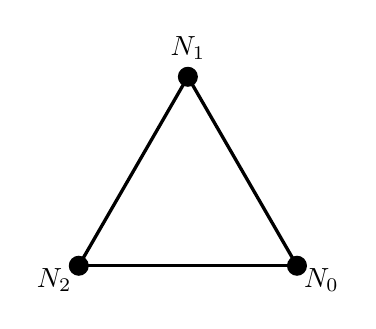
\begin{tikzpicture}[scale=0.8]
                    \foreach \n in {0,...,2}{
                        \draw[very thick] ({-120*\n-30}:2)--({-120*(\n+1)-30}:2) node[midway,sloped,allow upside down]{$\blacktriangleright\blacktriangleright\blacktriangleright$};
                        \draw[fill=black] ({-120*\n-30}:2) circle[radius=0.15];
                    }
                    \draw (-30:2.45) node{$N_0$};
                    \draw (90:2.45) node{$N_1$};
                    \draw (210:2.45) node{$N_2$};
                \end{tikzpicture}
                \caption{Quiver of the $\C^3/\Z_3$ daughter theory.}
                \label{fig:Z3quiver}
            \end{figure}
            The adjacency matrix of this quiver is
            \begin{equation}
                A=
                \begin{bmatrix}
                    0 & 3 & 0 \\
                    0 & 0 & 3 \\
                    3 & 0 & 0
                \end{bmatrix}
            \end{equation}
            which is coherent with the fact that the coefficients of the McKay decomposition of $\rho_1\oplus\rho_1\oplus\rho_1$ are
            \begin{align}
                \begin{split}
                    n_{00} &= 0,\quad n_{01} = 3\qquad n_{02}=0,\\
                    n_{10} &= 0,\quad n_{11} = 0,\qquad n_{12}=3,\\
                    n_{20} &= 3,\quad n_{21} = 0,\qquad n_{22}=0.
                \end{split}
            \end{align}

        \subsubsection{Gauge anomaly cancellation}
        
            We get the three following conditions:
            \begin{align}
                \SU(N_0) &: N_2-N_1 = 0,\\
                \SU(N_1) &: N_0-N_2 = 0,\\
                \SU(N_2) &: N_1-N_0 = 0.
            \end{align}
            which immediately imply
            \begin{equation}
                N_0=N_1=N_2.
            \end{equation}
            From \eqref{eq:sumNiZ3}, we get that $N_0=N_1=N_2=N/3$, meaning that that the daughter theory has quantum gauge symmetry if and only if the parent theory with has gauge group $\SU(N)$ where $N$ is a multiple of $3$. Or, in other words, if the number of D-branes is a multiple of $3$.

    \subsection{$(p+1)$-dimensional quiver gauge theories}

        Let us mention that we can generalize our initial brane-world paradigm and consider D$p$-branes in type II string theory (type IIA if $p$ is even and type IIB if $p$ is odd) instead of just D$3$-branes. The spacetime is then of the form
        \begin{equation}
            M = \R^{1,p}\times\R^{9-p}/\Gamma
        \end{equation}
        where $\Gamma$ is a discrete subgroup of $\Spin(9-p)$. If $\Gamma$ is a subgroup of a special holonomy group, we recover a somewhat generalized version of the paradigm that we discussed above. In this case the transverse space is a Calabi-Yau orbifold and some degree of supersymmetry is preserved. Note that the fermionic and bosonic quivers that coincides. If $\Gamma$ is not a subgroup of a special holonomy group, then the $(p+1)$-dimensional quiver gauge theory that we obtain in the low-energy limit is not supersymmetric. We then have different quivers for the fermions and the bosons, although with the same vertices, by definition.

        Recall that the fraction of supercharges that is preserved by compactifying on a Calabi-Yau $n$-fold (with $\SU(n)$ holonomy) is $2^{1-n}$. Starting from the $\mN=2$ 10-dimensional type IIB string theory with 32 supercharges, this means that
        \begin{itemize}
            \item if we compactify on a $1$-fold, we get $32$ supercharges in $8$ dimensions so $\mN=2$,
            \item if we compactify on a $2$-fold, we get $16$ supercharges in $6$ dimensions so $\mN=2$,
            \item if we compactify on a $3$-fold, we get $8$ supercharges in $4$ dimensions so $\mN=2$,
            \item is we compactify on a $4$-fold, we get $4$ supercharges in $2$ dimensions so $\mN=4$.
        \end{itemize}

        We will however mostly mostly consider $4$-dimensional quiver gauge theories, i.e. living on D$3$-branes.
    

\section{$\mN=2$ daughter theories}\label{sec:N2QGT}

    %Let us consider that $\Gamma$ is a finite subgroup of $\SU(2)\subset\SU(3)$. It naturally acts on $\C^3$ trough its fundamental representation $\bs{2}$ as $\bs{1}\oplus\bs{2}$ (only acts on 2 coordinates).

    \subsection{$S=\C\times\C^2/\Z_n$}

        We consider a representation $(\rho,\C^N)$ of $\Z_n$. We decompose it on the set of irreducible representations of $\Z_n$ as
        \begin{equation}
            (\rho,\C^n)=\bigoplus^{n-1}_{i=0}N_i(\rho_i,\C).
        \end{equation}
        In other words, it is equivalent to the representation
        \begin{equation}
            \rho(g)=
            \begin{bmatrix}
                1 & & & \cdots & & & 0 \\
                & \ddots & & & & & \\
                & & 1 & & & &  \\
                \vdots & & & \ddots & & & \vdots \\
                & & & & \zeta^{n-1}_n & & \\
                & & & & & \ddots & \\
                0 & & & \cdots & & & \zeta^{n-1}_n 
            \end{bmatrix}
            \hspace{-0.2cm}
            \begin{tabular}{l}
            $\left.\lefteqn{\phantom{
                \begin{matrix}
                    a_0\\ \ddots\\ a_0\ 
                \end{matrix} 
            }}\right\}N_0$\\
            \vdots \\
            $\left.\lefteqn{\phantom{
                \begin{matrix}
                    b_0\\ \ddots\\ b_0\ 
                \end{matrix}
            }} \right\}N_{n-1}$
            \end{tabular}.\label{eq:reprrhoZn}
        \end{equation}
        Since $\dim\rho_i=1$, $\sum_i N_i=N$. 

        The gauge field configurations that are left invariant under the action of $\Z_n$ are therefore the ones that satisfy
        \begin{equation}
            \rho(g)A_\mu\rho(g)^{-1}=A_\mu.
        \end{equation}
        The constrained is easily solved by using the bi-index notation:
        \begin{equation}
            A_{\mu;i\alpha_i,i\beta_j}\mapsto \rho_i(g)A_{\mu;i\alpha_i,j\beta_j}\rho_j(g)^{-1}=\zeta^{i-j}_nA_{\mu;i\alpha_i,j\beta_j}.
        \end{equation}
        thus only the configurations with $A_{\mu;i\alpha_i,j\beta_j}=0$ if $i\neq j$ are invariant. The gauge field has therefore a block diagonal form:
        \begin{equation}
            A_\mu=
            \begin{bmatrix}
                A_{\mu;00} & & & \\
                & A_{\mu;11} & & \\
                & & \ddots & \\
                & & & A_{\mu;n-1,n-1}
            \end{bmatrix}
        \end{equation}
        with $A_{\mu;ij}\equiv (A_{\mu;i\alpha_i,j\beta_j})_{\alpha_i=0,\dots,N_i,\beta_j=0,\dots,N_j}$. The block $A_{ii}$ transforms under $\Z_n$ as $(\rho_i,V_i)^{N_i}$. For now it is only a simple generalization of the case $\C^3/\Z_3$. This makes sense: projection of the gauge field only depends the discrete group $\Gamma$, not on the way it acts on $\C^3$ because it does not transform under R-symmetry.
        
        The gauge group is now broken to
        \begin{equation}
            G_{\text{proj}}=\prod^{n-1}_{i=0}~\U(N_i).
        \end{equation}

        Now for the scalar fields. The action of $\Z_n$ that we consider leaves the first component of $\C^3$ untouched so we take the action $\boldsymbol{1}\oplus\boldsymbol{2}$ where $\boldsymbol{2}$ is the usual action of $\Z_n$ on $\C^2$. In other words, 
        \begin{equation}
            R(g)=
            \begin{bmatrix}
                1 & 0 & 0 \\
                0 & \zeta_n & 0 \\
                0 & 0 & \zeta^{-1}_n
            \end{bmatrix}.
        \end{equation}
        Or, equivalently, $R(g)\indices{^m_n}=\delta\indices{^m_n}A_n$ with $A_m=(1,1,\zeta_n,\zeta_n,\zeta^{-1}_n,\zeta^{-1}_n)$. The scalar field configurations that are left invariant satisfy
        \begin{equation}
            R(g)\indices{^m_n}\rho(g)X^n\rho(g)^{-1}=X^m
        \end{equation}
        for all $g\in\Z_n$. Using the bi-index notations, this becomes
        \begin{align}
            X^m_{i\alpha_i,j\beta_j}\mapsto  \delta\indices{^m_n}A_n\rho_i(g)X^m_{i\alpha_i,j\beta_j}\rho_j(g)^{-1}  = \delta\indices{^m_n}A_n\zeta^{i-j}_n X^m_{i\alpha_i,j\beta_j} =
            \begin{cases}
                \zeta^{i-j}_nX^m_{i\alpha_i,j\beta_j},\quad m=0,1\\
                \zeta^{i-j+1}_nX^m_{i\alpha_i,j\beta_j},\quad m=2,3\\
                \zeta^{i-j-1}_nX^m_{i\alpha_i,j\beta_j},\quad m=4,5\\
            \end{cases}\\
            \bar{X}^m_{i\alpha_i,j\beta_j}\mapsto \delta\indices{^m_n}\bar{A_n}\rho_i(g)\bar{X}^m_{i\alpha_i,j\beta_j}\rho_j(g)^{-1}  = \delta\indices{^m_n}\bar{A_n}\zeta^{i-j}_n X^m_{i\alpha_i,j\beta_j} =
            \begin{cases}
                \zeta^{i-j}_nX^m_{i\alpha_i,j\beta_j},\quad m=0,1\\
                \zeta^{i-j-1}_nX^m_{i\alpha_i,j\beta_j},\quad m=2,3\\
                \zeta^{i-j+1}_nX^m_{i\alpha_i,j\beta_j},\quad m=4,5\\
            \end{cases}
        \end{align}
        thus only the configurations with $X^{0,1}_{i\alpha_i,j\beta_j}=0$ if $i-j\neq0$, $X^{2,3}_{i\alpha_i,j\beta_j}=0$ if $i-j+1\neq0$ and $X^{4,5}_{i\alpha_i,j\beta_j}=0$ if $i-j-1\neq0$ are left invariant (and similarly for the conjugated fields). The scalar fields $X$ have a the following forms:
        {\small
        \begin{align}
            X^{0,1}&=
            \begin{bmatrix}
                X^{0,1}_{00} &  & 0 \\
                 & \ddots & \\
                0 & & X^{0,1}_{n-1,n-1}
            \end{bmatrix},\\
            X^{2,3}&=
            \begin{bmatrix}
                0 & X^{2,3}_{01} & & 0 \\
                 & \ddots & \ddots & \\
                 & & 0 & X^{2,3}_{n-2,n-1} \\
                X^{2,3}_{n-1,0} & & & 0 
            \end{bmatrix},\quad
            X^{4,5}=
            \begin{bmatrix}
                0 & & & X^{4,5}_{0,n-1} \\
                X^{4,5}_{10} & 0 & & \\
                 & \ddots & \ddots  & \\
                0 & & X^{4,5}_{n-1,n-2} & 0
            \end{bmatrix},\\
            \bar{X}^{0,1}&=
            \begin{bmatrix}
                \bar{X}^{0,1}_{00} &  & 0 \\
                 & \ddots & \\
                0 & & \bar{X}^{0,1}_{n-1,n-1}
            \end{bmatrix},\\
            \bar{X}^{2,3}&=
            \begin{bmatrix}
                0 & & & \bar{X}^{2,3}_{0,n-1} \\
                \bar{X}^{2,3}_{10} & 0 & & \\
                 & \ddots & \ddots  & \\
                0 & & \bar{X}^{2,3}_{n-1,n-2} & 0
            \end{bmatrix},\quad
            \bar{X}^{4,5}=
            \begin{bmatrix}
                0 & \bar{X}^{4,5}_{01} & & 0 \\
                 & \ddots & \ddots & \\
                 & & 0 & \bar{X}^{4,5}_{n-2,n-1} \\
                 \bar{X}^{4,5}_{n-1,0} & & & 0
            \end{bmatrix}
        \end{align}}
        so $X^m_{ij}$ is an $N_i\times N_j$ block and transforms under the representation $(\boldsymbol{\textbf{N}_i},\boldsymbol{\bar{\textbf{N}}_j})$ of $\U(N_i)\times\U(N_j)$:
        \begin{align}
            X^{0,1}_{i,i} &\in \boldsymbol{\textbf{N}_i}\otimes\boldsymbol{\bar{\textbf{N}}_i} \cong \Hom(V_i,V_i),\\
            X^{2,3}_{i,i+1} &\in \boldsymbol{\textbf{N}_{i+1}}\otimes\boldsymbol{\bar{\textbf{N}}_i} \cong \Hom(V_{i+1},V_i),\\
            X^{4,5}_{i+1,i} &\in \boldsymbol{\textbf{N}_i}\otimes\boldsymbol{\bar{\textbf{N}}_{i+1}} \cong \Hom(V_i,V_{i+1}).
        \end{align}
        So the scalar fields are split up in three families depending on the way they transform under R-symmetry. We now see a big difference with the case $\C^3/\Z_3$: since the R-symmetry does not act the same way on each directions in $\C^3$, the invariant scalar field configurations are not the same in each direction either.

        Let us draw the quiver for the case $n=3$ so that we can compare to \ref{fig:Z3quiver}. We have $2\cdot 9=18$ real scalar fields in $9$ different representations:
        \begin{align}
            X^0_{00},X^1_{00}&\in(\boldsymbol{\textbf{N}_0},\boldsymbol{\bar{\textbf{N}}_0}),\quad
            X^0_{11},X^1_{11}\in(\boldsymbol{\textbf{N}_1},\boldsymbol{\bar{\textbf{N}}_1}),\quad
            X^0_{22},X^1_{22}\in(\boldsymbol{\textbf{N}_2},\boldsymbol{\bar{\textbf{N}}_2}),\\
            X^2_{01},X^3_{01}&\in(\boldsymbol{\textbf{N}_1},\boldsymbol{\bar{\textbf{N}}_0}),\quad
            X^2_{12},X^3_{12}\in(\boldsymbol{\textbf{N}_2},\boldsymbol{\bar{\textbf{N}}_1}),\quad
            X^2_{20},X^3_{20}\in(\boldsymbol{\textbf{N}_0},\boldsymbol{\bar{\textbf{N}}_2}),\\
            X^4_{10},X^5_{10}&\in(\boldsymbol{\textbf{N}_0},\boldsymbol{\bar{\textbf{N}}_1}),\quad
            X^4_{21},X^5_{21}\in(\boldsymbol{\textbf{N}_1},\boldsymbol{\bar{\textbf{N}}_2}),\quad
            X^4_{02},X^5_{02}\in(\boldsymbol{\textbf{N}_2},\boldsymbol{\bar{\textbf{N}}_0}),
        \end{align}
        We now only have 1 complex scalar in each representation and the quiver is given by \ref{fig:2Z3quiver}.
        \begin{figure}[H]
            \centering
            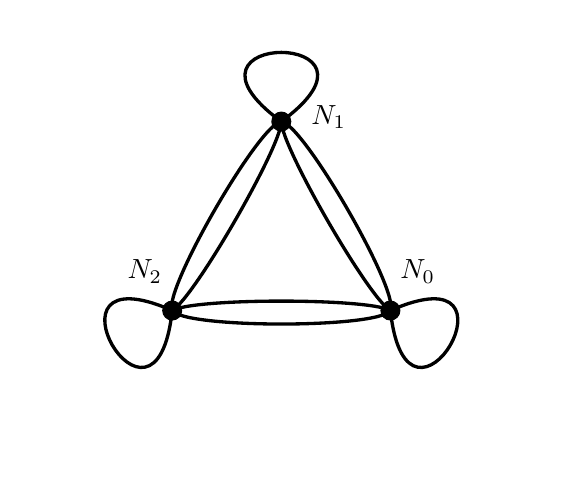
\begin{tikzpicture}[scale=0.8]
                \foreach \n in {0,...,2}{
                    \draw[very thick] ({120*\n-30}:2) .. controls ({120*\n-20}:2) and ({120*\n+120-40}:2) .. ({120*\n+120-30}:2) node[midway,sloped,allow upside down]{$\blacktriangleright$};
                    \draw[very thick] ({120*\n-30}:2) .. controls ({120*\n-30}:1.6) and ({120*\n+120-30}:1.6) .. ({120*\n+120-30}:2) node[midway,sloped,allow upside down]{$\blacktriangleleft$};
                    \draw[very thick] ({120*\n-30}:2) .. controls ({120*\n}:4) and ({120*\n-60}:4) .. ({120*\n-30}:2) node[midway,sloped,allow upside down]{$\blacktriangleright$};
                    \draw[fill=black] ({120*\n-30}:2) circle[radius=0.15];
                }
                \draw (-10:2.2) node{$N_0$};
                \draw (70:2.2) node{$N_1$};
                \draw (190:2.2) node{$N_2$};
            \end{tikzpicture}
            \caption{Quiver of the $\C\times\C^2/\Z_3$ daughter theory.}
            \label{fig:2Z3quiver}
        \end{figure}
        It is easy to see how the construction of the the quiver generalizes for arbitrary $n$. The adjacency matrix is
        \begin{equation}
            A=
            \begin{bmatrix}
                1 & \cdots & 1 \\
                \vdots & \ddots & \vdots \\
                1 & \cdots & 1
            \end{bmatrix}
        \end{equation}
        which is, as it should, coincides with the McKay decomposition of $\boldsymbol{1}\oplus\boldsymbol{2}$:
        \begin{align}
            \begin{split}
                n_{00} &= 1,\quad\dots,\qquad n_{0,n-1}=1,\\
                &\vdots\hspace{3.7cm}\vdots\\
                n_{n-1,0} &= 1,\quad\dots,\qquad n_{n-1,n-1}=1.
            \end{split}
        \end{align}
        
        Gauge anomaly cancellation now imposes that
        \begin{equation}
            N_{i-1}-N_{i-1}+N_{i+1}+N_{i+1}=0
        \end{equation}
        for $i=0,\dots,n-1$. Those constrains are always satisfied so the the factors $N_i$ are arbitrary, as long as $\sum_iN_i=N$ of course.

        This quiver is easy to scale up for any $n$. We therefore implement that into Mathematica and get the quivers for any $n$.

    \subsection{$S=\C\times\C^2/\D_n$}

        We quotient $\C^3$ by the binary dihedral group $\D_n$ that acts on the last two components. A set of irreducible representations of $\D_n$ is given by
        \begin{equation}
            \{(\rho_i,V_i)\}_{i=0,\dots,n+2}
        \end{equation}
        with $V_i=\C$ for $i=0,\dots,3$ and $V_i=\C^2$ for $i=4,\dots,n+2$, so there are $4$ one-dimensional representations and $n-1$ two-dimensional representations. They are explicitely given in section \ref{sec:irrep}. Any representation of $(\rho,\C^N)$ of $\D_n$ can be decomposed as
        \begin{equation}
            ()
        \end{equation}
        
        Using the bi-index notations $A_{\mu;i\alpha_i,j\beta_j}$ with $i,j=0,\dots,n+2$ and $\alpha_i,\beta_j=0,\dots,N_i\dim\rho_i-1$, the invariant configurations must have $A_{\mu;ij}=0$ if $i\neq j$, i.e. it must have a diagonal block-form, wiht block of size $N_i\times N_i$ for $i=0,\dots,3$ and of size $2N_i\times 2N_i$ for $i=4,\dots,n+1$. The blocks transforming under the $2$-dimensional representations must have the form
        \begin{equation}
            A_{\mu;ii}=
            \begin{bmatrix}
                A_{\mu;i0,i0} & A_{\mu;i0,i1} & \cdots & A_{\mu;i,0,i,2N_i-2} & A_{\mu;i,0,i,2N_i-1} \\ 
                \mp A_{\mu;i0,i1} & A_{\mu;i0,i0} & \cdots & \mp A_{\mu;i,0,i,2N_i-1} & A_{\mu;i,0,i,2N_i-2} \\
                \vdots & \cdots & \ddots & \vdots & \vdots \\
                A_{\mu;i,2N_i-2,i,0} & A_{\mu;i,2N_i-2,i1} & \cdots & A_{\mu;i,2N_i-2,i,2N_i-2} & A_{\mu;i,2N_i-2,i,2N_i-1} \\ 
                \mp A_{\mu;i,2N_i-2,i1} & A_{\mu;i,N_i-2,i,0} & \cdots & \mp  A_{\mu;i,2N_i-2,i,2N_i-1} & A_{\mu;i,2N_i-2,i,2N_i-2}
            \end{bmatrix}
        \end{equation}
        so each block is composed of $N^2_i$ $2\times2$ matrices of the form
        \begin{equation}
            \begin{bmatrix}
                A & B \\
                \mp B & A
            \end{bmatrix}.
        \end{equation}
        We take the ``$-$'' signs when $i$ is even and the ``$+$'' signs when $i$ is odd. This comes from the fact that the $2$-dimensional representations involve alternating signs.

        R-symmetry acts on the three complex scalar fields as
        \begin{equation}
            R(A) =
            \begin{matrix}
                A
            \end{matrix}
        \end{equation}

        \marker

    \subsection{$S=\C\times\C^2/\T,\mathcal{O},\I$}

        \marker




\section{$\mN=1$ daughter theories}

    \subsection{$S=\C^3/\Z_n$}

        Let us now consider the general case of $\Z_n$ acting on $\C^3$, i.e. we want to generalize the case that we treated in section \ref{sec:C3Z3}. 
        
        \subsubsection{Actions of $\Z_n$ on $\C^3$}
        
            The first thing to do is to specify a representation of $\Z_n$ on $\C^3$. Any representation $(R,\C^3)$ can be decomposed as
            \begin{equation}
                R=\bigoplus^{n-1}_{k=0} \rho^{\oplus n_k}_k
            \end{equation}
            and is therefore equivalent to a block-diagonal representation. This implies that $\sum_kn_k=3$ so $R$ can always be written as
            \begin{equation}
                R(g)= (\rho_a\oplus\rho_b\oplus\rho_c)(g)=
                \begin{bmatrix}
                    \zeta^a_n & 0 & 0 \\
                    0 & \zeta^b_n & 0 \\
                    0 & 0 & \zeta^c_n
                \end{bmatrix}\label{eq:reprZnC3}
            \end{equation}
            with $a,b,c$ some arbitrary exponents. We denote the representation \eqref{eq:reprZnC3} by $(a,b,c)$. Let us make a few remarks on these representations:
            \begin{itemize}
                \item Since we consider $\Z_n$ as a subgroup of $\SU(3)$, we must have
                \begin{equation}
                    (a+b+c)\mod n = 0\label{eq:cdtabc}
                \end{equation}
                such that $\det(R(g))=1$.
                \item Taking $a$ or $a+n$ gives the same representation and the same is true for $b$ and $c$, so we we can actually restrict ourselves to $0<a,b,c<n$. We can trade the strict inequalities and allow the values $0$ or $n$ if we want to consider trivial representations as well. In this case, we will find that at least one direction of $\C^3$ is left untouched, i.e. we are in the situation where the orbifold is actually $\C\times\C^2/\Z_n$, which we will not consider here.
                \item Permuting $a,b,c$ gives equivalent representations so we can take $a,b,c$ to be ordered, so $0<a\leq b\leq c<n$.
            \end{itemize}

            The problem has now been reformulated as follows:
            we are looking for all possible ordered triplets $(a,b,c)$ such that $0<a\leq b\leq c<n$ and \eqref{eq:cdtabc}. For $n=1$ and $n=2$, it is clear that this is not possible, the possibilities involve at least one trivial representation. For $n=3$, the only possibility is $(1,1,1)$, the one we used in \ref{sec:C3Z3}. What about bigger values of $n$? First, note that $0<a\leq b\leq c<n$ implies that the maximum value of $a+b+c$ is $3n-1$. From equation \eqref{eq:cdtabc}, the only two possibilities are then $a+b+c=n$ or $a+b+c=2n$. What simplifies the analysis is that the second case can actually be ignored because it is already being taken care of by the first case. Let us explain that in more details: \marker
            
            Now that we have seen that the only possibility is $a+b+c=n$, we find that the maximum value that $a$ can take is $\lfloor n/3\rfloor$, so $a=1,\dots,\lfloor n/3\rfloor$. $c$ can then be expressed in terms of $a$ and $b$ as $c=n-a-b$. The constraint $b\leq c$ then implies $b\leq (n-a)/2$, i.e. $b=a,\dots,\lfloor (n-a)/2\rfloor$. To summarize, the representations are all the representations of the form
            \begin{equation}
                (a,b,n-a-b)
            \end{equation}
            with $a=1,\dots,\lfloor n/3\rfloor$ and $b=a,\dots,\lfloor (n-a)/2\rfloor$. For small values, we get
            \begin{align*}
                \Z_1 &: \text{necessarily involves a trivial representation}\\
                \Z_2 &: \text{necessarily involves a trivial representation}\\
                \Z_3 &: (1,1,1)\\
                \Z_4 &: (1,1,2)\\
                \Z_5 &: (1,1,3),(1,2,2)\label{reprZ5C3}\marker\\
                \Z_6 &: (1,1,4),(1,2,3),(2,2,2)\\
                \Z_7 &: (1,1,5),(1,2,4),(1,3,3),(2,2,3)\marker\\
                &\vdots
            \end{align*}
            For an arbitrary $n$, the total number of different representation is
            \begin{equation}
                \sum^{\lfloor n/3\rfloor}_{a=1}~\left\lfloor \frac{n-3a}{2}+1\right\rfloor = \begin{cases}
                    3k^2,\qquad\text{if $n=6k$}\\
                    3k^2+k,\qquad\text{if $n=6k+1$},\\
                    3k^2+2k,\qquad\text{if $n=6k+2$},\\
                    3k^2+3k+1,\qquad\text{if $n=6k+3$},\\
                    3k^2+4k+1,\qquad\text{if $n=6k+4$},\\
                    3k^2+5k+2,\qquad\text{if $n=6k+5$}
                \end{cases}
            \end{equation}
            The details are presented in appendix \ref{app:compsum}.

        \subsubsection{Example: $\Z_5$}

            For $\Z_5$, we saw that there are two nonequivalent ways of acting on $\C^3$, see \eqref{reprZ5C3}. Let us first consider the action $(1,1,3)$
            \begin{equation}
                R(g)=
                \begin{bmatrix}
                    \zeta_5 & 0 & 0\\
                    0 & \zeta_5 & 0\\
                    0 & 0 & \zeta^3_5
                \end{bmatrix}
            \end{equation}
            i.e. $R=\rho_1\oplus\rho_1\oplus\rho_3$.

            For the gauge field, the reasoning is exactly the same than for $\Z_3$ and we get
            \begin{equation}
                A_\mu=
                \begin{bmatrix}
                    A_{\mu;00} & & \\
                    & \ddots & \\
                    & & A_{\mu;44}
                \end{bmatrix}
            \end{equation}
            where each block $A_{\mu;ii}$ is of size $N_i\times N_i$. The projected gauge group is
            \begin{equation}
                G_{\text{proj}} = \U(N_0)\times\U(N_1)\times\U(N_2)\times\U(N_3)\times\U(N_4).
            \end{equation}

            The scalar fields transform as
            \begin{equation}
                X^m_{i\alpha_i,j\beta_j}\to R(g)\indices{^m_n}\rho_i(g)X^n_{i\alpha_i,j\beta_j}\rho_j(g)^{-1}
            \end{equation}
            so the invariant configurations must satisfy
            \begin{equation}
                X^m_{i\alpha_i,j\beta_j} = R(g)\indices{^m_n}\zeta^{i-j}_4\rho_i(g)X^n_{i\alpha_i,j\beta_j} = 
                \begin{cases}
                    \zeta^{i-j+1}X^m_{i\alpha_i,j\beta_j},\quad\text{if } m=0,1,2,3\\
                    \zeta^{i-j+3}X^m_{i\alpha_i,j\beta_j},\quad\text{if } m=4,5.
                \end{cases}
            \end{equation}
            and are therefore of the form
            \begin{equation}
                X^m = 
                \begin{bmatrix}
                    0 & X^m_{01} & 0 & 0 & 0\\
                    0 & 0 & X^m_{12} & 0 & 0\\
                    0 & 0 & 0 & X^m_{23} & 0\\
                    0 & 0 & 0 & 0 & X^m_{34}\\
                    X^m_{40} & 0 & 0 & 0 & 0
                \end{bmatrix}
            \end{equation}
            for $m=0,1,2,3$ and 
            \begin{equation}
                X^m = 
                \begin{bmatrix}
                    0 & 0 & 0 & X^m_{03} & 0\\
                    0 & 0 & 0 & 0 & X^m_{14}\\
                    X^m_{20} & 0 & 0 & 0 & 0\\
                    0 & X^m_{31} & 0 & 0 & 0\\
                    0 & 0 & X^m_{42} & 0 & 0
                \end{bmatrix}
            \end{equation}
            for $m=4,5$. Gauge anomaly cancellation imposes
            \begin{align}
                -N_{i-2}+N_{i+2}-2N_{i+1}+2N_{i-1}=0
            \end{align}
            for $i=0,1,2,3,4$ which implies that
            \begin{equation}
                N_0=N_1=N_2=N_3=N_4.
            \end{equation}

            Now if we choose the representation $(1,2,2)$, i.e.
            \begin{equation}
                R(g)=
                \begin{bmatrix}
                    \zeta_5 & 0 & 0\\
                    0 & \zeta^2_5 & 0\\
                    0 & 0 & \zeta^2_5
                \end{bmatrix}
            \end{equation}
            we get instead that the invariant field configurations must satisfy
            \begin{equation}
                X^m_{i\alpha_i,j\beta_j} = R(g)\indices{^m_n}\zeta^{i-j}_4\rho_i(g)X^n_{i\alpha_i,j\beta_j} =
                \begin{cases}
                    \zeta^{i-j+1}X^m_{i\alpha_i,j\beta_j},\quad\text{if } m=0,1\\
                    \zeta^{i-j+2}X^m_{i\alpha_i,j\beta_j},\quad\text{if } m=2,3,4,5.
                \end{cases}
            \end{equation}
            and are therefore of the form
            \begin{equation}
                X^m = 
                \begin{bmatrix}
                    0 & X^m_{01} & 0 & 0 & 0\\
                    0 & 0 & X^m_{12} & 0 & 0\\
                    0 & 0 & 0 & X^m_{23} & 0\\
                    0 & 0 & 0 & 0 & X^m_{34}\\
                    X^m_{40} & 0 & 0 & 0 & 0
                \end{bmatrix}
            \end{equation}
            for $m=0,1$ and 
            \begin{equation}
                X^m = 
                \begin{bmatrix}
                    0 & 0 &  X^m_{02} & 0 & 0\\
                    0 & 0 & 0 &  X^m_{13} & 0\\
                    0 & 0 & 0 & 0 &  X^m_{24}\\
                    X^m_{30} & 0 & 0 & 0 & 0\\
                    0 &  X^m_{41} & 0 & 0 & 0
                \end{bmatrix}
            \end{equation}
            for $m=2,3,4,5$. Gauge anomaly cancellation imposes
            \begin{align}
                -2N_{i+2}+2N_{i-2}-N_{i+1}+N_{i-1}=0\marker
            \end{align}
            for $i=0,1,2,3,4$ which implies that
            \begin{equation}
                N_0=N_1=N_2=N_3=N_4.
            \end{equation}

            \begin{figure}
                \centering
                \begin{subfigure}[b]{0.3\textwidth}
                    \centering
                    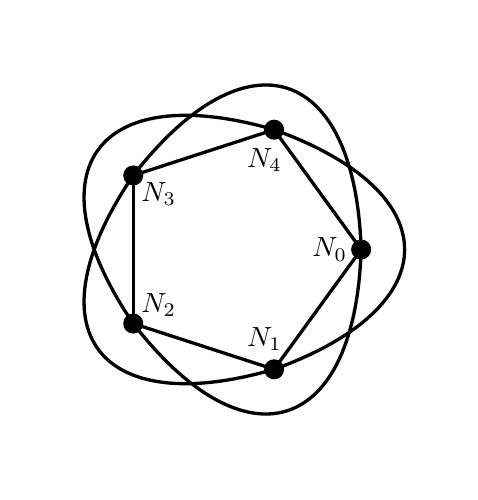
\begin{tikzpicture}[scale=0.8]
                        \foreach \n in {0,...,4}{
                            \draw[very thick] (-72*\n:2) .. controls ({-72*(\n+1)+15}:3.5) and ({-72*(\n+1)-15}:3.5) .. ({-72*(\n+2)}:2) node[midway,sloped,allow upside down]{$\blacktriangleright$};
                            \draw[very thick] ({-72*\n}:2) -- ({-72*(\n-1)}:2) node[midway,sloped,allow upside down]{$\blacktriangleright\blacktriangleright$};
                            \draw[fill=black] (-72*\n:2) circle[radius=0.15];
                            \draw (-72*\n:1.5) node{$N_\n$};
                        }
                    \end{tikzpicture}
                    \caption{$(1,1,3)$}
                    \label{fig:y equals x}
                \end{subfigure}
                \hspace{2cm}
                \begin{subfigure}[b]{0.3\textwidth}
                    \centering
                    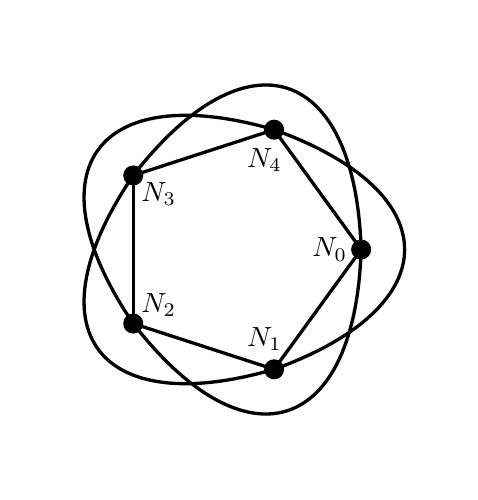
\begin{tikzpicture}[scale=0.8]
                        \foreach \n in {0,...,4}{
                            \draw[very thick] (-72*\n:2) .. controls ({-72*(\n+1)+15}:3.5) and ({-72*(\n+1)-15}:3.5) .. ({-72*(\n+2)}:2) node[midway,sloped,allow upside down]{$\blacktriangleleft\blacktriangleleft$};
                            \draw[very thick] ({-72*\n}:2) -- ({-72*(\n-1)}:2) node[midway,sloped,allow upside down]{$\blacktriangleright$};
                            \draw[fill=black] (-72*\n:2) circle[radius=0.15];
                            \draw (-72*\n:1.5) node{$N_\n$};
                        }
                    \end{tikzpicture}
                    \caption{$(1,2,2)$}
                    \label{fig:three sin x}
                \end{subfigure}
                \caption{Quivers of the $\C^3/\Z_5$ daughter theories.}
                \label{fig:Z5graphs}
           \end{figure}

           Note that, even we thought that $(1,1,3)$ and $(1,2,2)$ were different representation, that are actually equivalent in the sense that $(1,1,3)+(1,1,3)=(2,2,1)$. The two quivers in fig. \ref{fig:Z5graphs} should therefore be the same. And indeed, upon further inspection, the two are the same. To see this, we can rename the vertices in the second graph as $N_1\to N_3,N_2\to N_1,N_3\to N_4,N_4\to N_2$. This renaming defines the bijection between the two graphs. A more pragmatic way to see this is to look at the adjacency matrices:
           \begin{equation}
                a_{(1,1,3)}=
                \begin{bmatrix}
                    0 & 0 & 1 & 0 & 2 \\
                    2 & 0 & 0 & 1 & 0 \\
                    0 & 2 & 0 & 0 & 1 \\
                    1 & 0 & 2 & 0 & 0 \\
                    0 & 1 & 0 & 2 & 0
                \end{bmatrix}\qquad
                a_{(1,2,2)}=
                \begin{bmatrix}
                    0 & 0 & 0 & 2 & 1 \\
                    1 & 0 & 0 & 0 & 2 \\
                    1 & 1 & 0 & 0 & 0 \\
                    0 & 2 & 1 & 0 & 0 \\
                    0 & 0 & 2 & 1 & 0
                \end{bmatrix}.
           \end{equation}
           Changing the names of the vertices is equivalent to swapping line and columns. For example, 

        \subsubsection{General $\Z_n$}

           Let us now consider the general action
           \begin{equation}
                R(g)=
                \begin{bmatrix}
                    \zeta^a_n & 0 & 0\\
                    0 & \zeta^b_n & 0\\
                    0 & 0 & \zeta^c_n
                \end{bmatrix}
           \end{equation}
           of $\Z_n$ on $\C^3$, where $(a,b,c)$ one of the representation that we studied before. In particular, recall that $a+b+c=n$. Following the same reasoning than before, we get that the gauge field of of the form
           \begin{equation}
               A_\mu=
               \begin{bmatrix}
                   A_{\mu;00} & & \\
                   & \ddots & & \\
                   & & A_{\mu;n-1,n-1}
               \end{bmatrix}.
           \end{equation}

           Invariant scalar field configurations transform as
           \begin{equation}
               X^m_{i\alpha_i,j\beta_j}=
               \begin{cases}
                   \zeta^{i-j+a}_nX^m_{i\alpha_i,j\beta_j},\qquad \text{if }m=0,1\\
                   \zeta^{i-j+b}_nX^m_{i\alpha_i,j\beta_j},\qquad \text{if }m=2,3\\
                   \zeta^{i-j+c}_nX^m_{i\alpha_i,j\beta_j},\qquad \text{if }m=4,5
               \end{cases}
           \end{equation}
           so
           \begin{align}
               X^{0,1}_{j-a,j} &\in (\boldsymbol{\textbf{N}_j},\boldsymbol{\bar{\textbf{N}}_{j-a}}),\\
               X^{2,3}_{j-b,j} &\in (\boldsymbol{\textbf{N}_j},\boldsymbol{\bar{\textbf{N}}_{j-b}}),\\
               X^{4,5}_{j-c,j} &\in (\boldsymbol{\textbf{N}_j},\boldsymbol{\bar{\textbf{N}}_{j-c}})
           \end{align}
           are the only possible non-vanishing components. This allows us to quickly draw all the possible quivers for a given $n$. Once again, the difficulty is only computational, not conceptual. This can therefore easily be implemented into Mathematica and we get the quiver for any $n$ and any representation $(a,b,c)$.
        
    \subsection{$S=\C^3/\Delta(3n^2),\Delta(6n^2)$}

    \subsection{$S=\C^3/\Sigma_{36\times 3},\Sigma_{60\times 3},\Sigma_{168\times 3},\Sigma_{216\times 3},\Sigma_{360\times 3}$}

    \subsection{$S=\C^3/(\Z_m\times\Z_n)$}

        \subsubsection{Representations of $\Z_m\times\Z_n$}

           We consider the group $\Z_m\times\Z_n$. Let us denote by $\{\mu_i\}_{i=0,\dots,m-1}$ and $\{\sigma_j\}_{j=0,\dots,n-1}$ two complete set of irreducible representation of $\Z_m$ and $\Z_n$ respectively, with
           \begin{align}
               \mu(g_1)&=\zeta^i_m\\
               \sigma_j(g_2)&=\zeta^j_n
           \end{align}
           where $g_1$ and $g_2$ are the generating elements of $\Z_m$ and $\Z_n$ respectively. $\Z_m\times\Z_n$ is of order $mn$ and possesses the same number of equivalency classes (abelian). It has therefore $mn$ irreducible representations. Since the group is abelian, they are all of dimension $1$. Let us denote by $\{T_k\}_{k=0,\dots,m+n-1}$ a complete set of irreducible representations. Since we have a product group, for any $k$ there exists indices $i(k)$ and $j(k)$ such that $T_k=\mu_{i(k)}\otimes\sigma_{j(k)}$. We choose the indices $i(k)$ and $j(k)$ such that
           \begin{align*}
               T_0 &= \mu_0\otimes\mu_0,\\
               T_1 &= \mu_0\otimes\mu_1,\\
               T_2 &= \mu_0\otimes\mu_2,\\
               &\vdots\\
               T_{n-1} &= \mu_0\otimes\mu_{n-1},\\
               T_n &= \mu_1\otimes\mu_0,\\
               &\vdots\\
               T_{2n-1} &= \mu_1\otimes\mu_{n-1},\\
               &\vdots\\
               T_{mn-1} &= \mu_{m-1}\otimes\mu_{n-1}.
           \end{align*}
           That is, we take
           \begin{equation}
               \begin{cases}
                   i(k) &= \lfloor k/n\rfloor\\
                   j(k) &= k\mod n
               \end{cases}\qquad \Leftrightarrow \qquad k=i(k)n+j(k).
           \end{equation}
           Note that this simply a dictionary between a line notation and a matrix notation and that it is indeed a bijection $k\Leftrightarrow i,j$. In this way, we can proceed to similar manipulations than before, were we used line notations. 

           Any representation $R$ of $\Z_m\times\Z_n$ can be decomposed as
           \begin{equation}
               R=\bigoplus_{i,j}N_k T_k=\bigoplus_{i,j}N_{ij}(\mu_{i}\otimes\sigma_{j})
           \end{equation}
           with $N_k=N_{i(k)j(k)}$. We must have $\sum_kN_k=3$. In other words, any representation of $\Z_m\times\Z_n$ on $\C^3$ is equivalent to
           \begin{equation}
                R(g_1,g_2)=[(\mu_{a}\otimes\sigma_{a'})\oplus(\mu_{b'}\otimes\sigma_{b'})\oplus(\mu_{c}\otimes\sigma_{c'})](g_1,g_2)=
               \begin{bmatrix}
                   \xi^a_m\xi^{a'}_n & 0 & 0 \\
                   0 & \xi^b_m\xi^{b'}_n & 0 \\
                   0 & 0 & \xi^c_m\xi^{c'}_n
               \end{bmatrix}.
           \end{equation}
           The determinant condition is
           \begin{align}
                \xi^{a+b+c}_m &= \xi^{-a'-b'-c'}_n\\
               \Leftrightarrow (a+b+c)\mod m &= (a'+b'+c')\mod n
           \end{align}

           

           \begin{equation}
            R(g_1,g_2)=
           \begin{bmatrix}
               \xi_m & 0 & 0 \\
               0 & \xi_n & 0 \\
               0 & 0 & \xi^{-1}_m\xi^{-1}_n
           \end{bmatrix}.
       \end{equation}

    \subsubsection{Projection}

        Let us start by the gauge field. We consider a unitary representation $(\rho,\C^N)$ of $\Z_m\times \Z_n$ on $\C^n$ and decompose it as
        \begin{equation}
            \rho=\bigoplus_{i,j}N_k T_k
        \end{equation}
        such that
        \begin{equation}
            \rho(g)=
            \begin{bmatrix}
                T_0(g) & & & \cdots & & & 0 \\
                & \ddots & & & & & \\
                & & T_0(g) & & & &  \\
                \vdots & & & \ddots & & & \vdots \\
                & & & & T_{mn-1}(g) & & \\
                & & & & & \ddots & \\
                0 & & & \cdots & & & T_{mn-1}(g) 
            \end{bmatrix}
            \hspace{-0.2cm}
            \begin{tabular}{l}
            $\left.\lefteqn{\phantom{
                \begin{matrix}
                    a_0\\ \ddots\\ a_0\ 
                \end{matrix} 
            }}\right\}N_0$\\
            \vdots \\
            $\left.\lefteqn{\phantom{
                \begin{matrix}
                    b_0\\ \ddots\\ b_0\ 
                \end{matrix}
            }} \right\}N_{mn-1}$
            \end{tabular}.
        \end{equation}

        We can now use our usual bi-index notation $A_{\mu;k\alpha_k,l\beta_l}$ with $k,l=0,\dots mn-1$ and $\alpha_k,\beta_k=0,\dots,N_k$ but instead it is more convenient to come back to our matrix notation by writing the block $A_{\mu;k,l}$ as $A_{\mu;i(k)j(k),i(l)j(l)}$ that we simply denote by $A_{\mu;ij,i'j'}$ with $i,i'\in\{0,\dots,n-1\}$ and $j,j'\in\{0,\dots,n-1\}$. So for $m=2,n=3$ for example, the link between the two notations is
        {\tiny
        \begin{equation}
            \begin{bmatrix}
                A_{\mu;00} & A_{\mu;01} & A_{\mu;02} & A_{\mu;03} & A_{\mu;04} & A_{\mu;05} \\
                A_{\mu;10} & A_{\mu;11} & A_{\mu;12} & A_{\mu;13} & A_{\mu;14} & A_{\mu;05} \\
                A_{\mu;20} & A_{\mu;21} & A_{\mu;22} & A_{\mu;23} & A_{\mu;24} & A_{\mu;05} \\
                A_{\mu;30} & A_{\mu;31} & A_{\mu;32} & A_{\mu;33} & A_{\mu;34} & A_{\mu;05} \\
                A_{\mu;40} & A_{\mu;41} & A_{\mu;42} & A_{\mu;43} & A_{\mu;44} & A_{\mu;05} \\
                A_{\mu;50} & A_{\mu;51} & A_{\mu;52} & A_{\mu;53} & A_{\mu;54} & A_{\mu;05}
            \end{bmatrix}=
            \begin{bmatrix}
                \begin{bmatrix}
                    A_{\mu;00,00} & A_{\mu;00,01} & A_{\mu;00,02}\\
                    A_{\mu;01,00} & A_{\mu;01,01} & A_{\mu;01,02}\\
                    A_{\mu;02,00} & A_{\mu;02,01} & A_{\mu;02,02}\\
                \end{bmatrix}
                \begin{bmatrix}
                    A_{\mu;00,10} & A_{\mu;00,11} & A_{\mu;00,12}\\
                    A_{\mu;01,10} & A_{\mu;01,11} & A_{\mu;01,12}\\
                    A_{\mu;02,10} & A_{\mu;02,11} & A_{\mu;02,12}\\
                \end{bmatrix}\\
                \begin{bmatrix}
                    A_{\mu;10,00} & A_{\mu;10,01} & A_{\mu;10,02}\\
                    A_{\mu;11,00} & A_{\mu;11,01} & A_{\mu;11,02}\\
                    A_{\mu;12,00} & A_{\mu;12,01} & A_{\mu;12,02}\\
                \end{bmatrix}
                \begin{bmatrix}
                A_{\mu;10,10} & A_{\mu;10,11} & A_{\mu;10,12}\\
                A_{\mu;11,10} & A_{\mu;11,11} & A_{\mu;11,12}\\
                A_{\mu;12,10} & A_{\mu;12,11} & A_{\mu;12,12}\\
            \end{bmatrix}
            \end{bmatrix}
        \end{equation}}
        So instead of considering $A_\mu$ to be a single $mn\times mn$ matrix of element $A_{\mu;kl}$, where $A_{\mu;kl}$ are $N_k\times N_l$ matrices, we consider it as an $m\times m$ where each element $A_{\mu,ii'}$ (line $i$ column $i'$) is itself an $n\times n$ matrices with elements $A_{\mu;ij,i'j'}$ (line $j$ column $j'$), as shown above.

        Using these notations, the gauge field transforms as
        \begin{equation}
            A_{\mu;ij,i'j'} \mapsto (\mu_i(g)\otimes\sigma_j(g))A_{\mu;ij,i'j'}(\mu_{i'}(g)\otimes\sigma_{j'}(g))^{-1} = \zeta^{i-i'}_m\zeta^{j'-j}_n A_{\mu;ij,i'j'}
        \end{equation}
        so invariant configurations can possess non-vanishing components $A_{\mu;ij,i'j'}$ only if
        \begin{align}
            \zeta^{i-i'}_m &= \zeta(j'-j)_n \\
            \Leftrightarrow\quad (i-i')\mod m &= (j'-j)\mod n \\
            \Leftrightarrow\quad j' &= j+\abs{i'-i}.
        \end{align}
        This means that the submatrices $A_{\mu;ii'}$ has an off-diagonal block form with offset $\abs{i'-i}$. Once again, for a general $n$, the difficulty is only computational, not conceptual. This can therefore easily be implemented into Mathematica and we get the form of the gauge field for any $n$.

        For the scalar fields, we have
        \begin{align}
            X^m_{ij,i'j'}&\mapsto R(g)\indices{^m_n}(\mu_i(g)\otimes\sigma_j(g))X^n_{ij,i'j'}(\mu_{i'}(g)\otimes\sigma_{j'}(g))^{-1}\\
            &\quad =
            \begin{cases}
                \zeta^{i-i'+1}_m\zeta^{j-j'}_n X^m_{ij,i'j'},\qquad m=0,1\\
                \zeta^{i-i'}_m\zeta^{j-j'+1}_n X^m_{ij,i'j'},\qquad m=2,3\\
                \zeta^{i-i'-1}_m\zeta^{j-j'-1}_n X^m_{ij,i'j'},\qquad m=4,5.
            \end{cases}
        \end{align}
        So a configuration is invariant if and only if the only non-vanishing component satisfy
        \begin{align}
            m=0,1 &: (i-i'+1)\mod m = (j'-j)\mod n\\
            m=2,3 &: (i-i')\mod m = (j'-j-1)\mod n\\
            m=4,5 &: (i-i'-1)\mod m = (j'-j+1)\mod n.
        \end{align}

\section{A note about projective representations, discrete torsion and deformations}

    \subsection{Projective representations and discrete torsion}

        Up until now, and in particular in all of our computations in section \ref{sec:orbsing}, we only considered ordinary representations, i.e. linear representations. We can however use a more general representations such as projective representations for example. That is, representations $\rho$ of $\Gamma$ such that for all $\gamma_1,\gamma_2\in\Gamma$,
        \begin{equation}
            \rho(\gamma_1)\rho(\gamma_2)=A(g_1,g_2)\rho(\gamma_1\gamma_2)
        \end{equation}
        for some factor $A(\gamma_1,\gamma_2)$. The $A(\gamma_1,\gamma_2)=1$ corresponding to linear representations. For consistency reasons, the factor $A(g_1,g_2)$ cannot be completely arbitrary and must a cocycle condition. As a result, the possibilities for $A(\gamma_1,\gamma_2)$ are classified by the second cohomology group $H^2(\Gamma,\C^*)$, also called \emph{discrete torsion}. There exists a projective representation if and only if the latter does not vanish. This new liberty, whenever admissible, provides new classes of quiver gauge theories that can be remarkably different from the ones we considered up until now, with no discrete torsion.

        What happens is that if one turns on an NSNS B-fiels alors the worldvolume, then the moduli space is expected to a non-commutative version of a Calabi-Yau space. This haw the discrete torsion is physically realized. Another, and actually equivalent through T-duality, way of studying gauge theories is to consider D-branes streched between configurations of NS$5$-branes\footnote{D$5$-branes are charged under the Ramond-Ramond field whose quanta comes from the Ramond-Ramond sector but NS$5$-branes are charges under the Kalb-Ramonf field whose quanta comes fromthe Neveu-Schwarz. On the worldvolume of an NS$5$-brane (6-dimensional) propagates propagates a superstring, this called the \emph{little string}.}. This is the\emph{Hanany-Witten setup}.

        The discrete tosrion also appears when writing the full open strin gpartition function that inclues the twisted sector where there is ambiguity up to a phase factor. As a consequence from modular invariance, the latter must satisfy certain cocycle conditions. It is precisely the deiscrete torsion. Note that this has been found to be true only for the open string sector.

    \subsection{Quiver gauge theories deformations and conifold}

        We can deforming the singular algebraic description of the orbifold with a field into a family smooth surfaces. The resulting total space is the \emph{conifold}.

\part{Toric singularities}

    The next best thing to orbifold singularities is the toric singularities.  The a specific class of supersymmetric gauge theories whose space of vacua is toric is called \emph{toric quiver gauge theories}. In this case, the inverse algorithm has been formalized in \cite{Feng_2001}.

\section{Toric geometry}

    The interest of toric varieties lies in the fact that all its defining data can be encoded in a simple auxilliary object called a fan. This data is purely combinatoric (discrete quantities) so complicated geometric problems are often reduced to simpler combinatorics problems.

    \subsection{Algebraic approach}

        \subsubsection{Cones}

            Let us consider a lattice $N=\Z^m$ and $N_\R=N\otimes\R$ the real vector space that we get by allowing real coefficients. Given $v_1,\dots,v_n$ of the lattice $N$, a \emph{cone}\footnote{More precisely, a strongly convex rational polyhedral cone.} $\sigma\subset N_\R$ is a the subset of the vector space $N_\R$ containing all points that are positive linear combination of the vectors $v_1,\dots,v_n$, that is
            \begin{equation}
                \sigma=\left\{\sum^n_{i=1}a_iv_i|a_i\geq0,a_i\in\R\right\}
            \end{equation}
            and such that $\sigma\cap(-\sigma)=\{0\}$. The last condition is the strong convexity condition and it imposes that our cone has to be ``acute''. The dimension of a cone is the dimension of $\Span(\sigma)$.
            
            The dual lattive $N^*$ of $N$ is the set of linear functionals on $L$ which take integer values on each point of $N$:
            \begin{equation}
                N^*=\{f\in(\Span(L))^*|\forall x\in N,f(x)\in\Z\}.
            \end{equation}
            We denote by $M$ the dual lattice of $N$ and by $M_\R$ the vector space we get from it by allowing real coefficients. For a given cone $\sigma$ in $ N_\R$, we can define the \emph{dual cone} $\sigma^\vee$ in $M_\R$ as
            \begin{equation}
                \sigma^\vee=\{m\in M_\R|\langle u,m\rangle\geq0,~ \forall u\in\sigma\}.
            \end{equation}

            Let us denote by $H_m$ the hyperplane gievn by the dual lattice point $m\in\sigma^\vee$: $H_m=\{v\in N_\R|\langle v,m\rangle=0\}$ and the closed halp-space $H^+_m=\{v\in N_\R|\langle v,m\rangle\geq0\}$. We then say that a hyperplane \emph{suports} a cone if the closed half-space of the hyperplane completely contains the cone. A \emph{face} of a cone is the intersection of the cone with a supporting hyperplane. Put differently, a convex subset $\tau$ is a face of $\sigma$ if and only whenever $u,v\in\sigma$ satisfy $u+v\in\tau$ then $i\in\tau$ and $v\in\tau$. Note that a hyper plane $H_m$ supports $\sigma$ if and only if $m\in\sigma^\vee$.

        \subsubsection{Toric varieties}

            An \emph{algebraic group} is a group that is also an algebraic variety and such the product and inversion are regular maps on the variety. Any product of $\C^*$ is an algebraic group that we call \emph{algebraic tori}. An affine variety $X\subset\C^n$ is a \emph{affine toric variety} if it contains the algebraic torus $\mathbb{T}=(\C^*)^n$ as a dense open subset such that the action of $\mathbb{T}$ on itself extends to an action $\mathbb{T}\times X\to X$ on $X$.

            \begin{examp*}
                Let us enumerate some examples of affine toric varieties.
                \begin{itemize}
                    \item $(\C^*)^n$ and $\C^n$ are naturally provided with an embeddingand an action of the torus and are toric varieties
                    \item $V=Z(x^3-y^2)$ with torus embedding
                    \begin{equation}
                        \left(
                        \begin{array}{ccc}
                            \C^* & \hookrightarrow & V \\
                            t & \longmapsto & (t^2,t^3))
                        \end{array}
                        \right).
                    \end{equation}
                    and the action $t\cdot(u,v)\mapsto(t^2u,t^3v)$.
                \end{itemize}
            \end{examp*}

            Generally speaking, an $n$-dimensional algebraic variety can be obtained as as particular holomorphic quotient of $\C^m$. If $\Z_\Delta\subset\C^m$ a set of points and $G\cong (\C^*)^{m-n}\times\Gamma$ is the group formed by the algebraic torus and an abelian discrete group $\Gamma$, then
            \begin{equation}
                X_\Delta=\frac{\{\C^m/\Z_\Delta\}}{G}.\label{eq:toricvargenform}
            \end{equation}

        \subsubsection{Toric variety of a cone}

            A \emph{semigroup} $S$ is a set with an internal associative $+$ operation and a neutral element $0$. It differs from a group in that elements need not have an inverse. A semigroup is \emph{affine} if it can be embedded as a subsemigroup in a lattice $\Z^m$ (\emph{integral}) and if there exists a finite set $\mathscr{A}$ such that $S=\N\mathscr{A}$ (\emph{finitely generated}). 
                
            What is interesting is that affine semigroups allows us to construct affine varities. For this, we need to introduce the notion of \emph{semigroup algebra} $\C[S]$ associated to any semi group $S$. It is the algebra generated by elements $\chi^u$ indexed by elements $u\in S$. The semigroup operation $+$ the induces a multiplication operation for the $\chi^u$ in $\C[S]$ as $\chi^u\cdot\chi^v=\chi^{u+v}$. For instance, the semigroup algebra of $S=\N^n$ is simply $\C[x_1,\dots,x_n]$ and the semigroup algebra of $S=\{2,3,\dots\}\subset\N$ is $\C[x,y]/I(x^3-y^2)$. The important result is now that if $S$ is an affine semigroup then $\Spec(\C[S])$ is an affine variety.

            Given a cone $\sigma$ and its dual cone $\sigma^\vee$, $S_\sigma=\sigma^\vee\cap M$ is finitely generated and hence an affine semigroup. In this way, we may obtain an affine variety from a cone as $U_\sigma=\Spec(\C[S_\sigma])$, this the \emph{variety if the cone} $\sigma$. An important result is that if $K[V]$ is the coordinate ring of an affine variety $V$, then $V=\Spec(K[V])$. From this, we see that $\C[S_\sigma]$ is exactly the coordinate ring of the variety $U_\sigma$ we are looking for.
            
            We have seen how to get an affine variety $U_\sigma$ from a cone $\sigma$. This variety is in fact toric. If $n$ denotes the rank of the lattice $\Z S_\sigma$, then there is torus action $\mathbb{T}=(\C^*)^n$ acting on $U_\sigma$. The torus that it contained is called the \emph{torus corresponding to a lattice} $N=\Z^m$ and is $\mathbb{Z}_N=(\C^*)^n$, so that the rank of the lattice equals the dimension of the torus:
            \begin{equation}
                T_N = N\otimes_\Z\C^*=\Hom_\Z(M,\C^*).
            \end{equation}
            To torus acts on $U_\sigma$ as $t\cdot\gamma:S_\sigma\to\C:m\mapsto\chi^m(t)\gamma(m)$, for all $t\in T_N$ and $\gamma\in\sigma$ (so$\gamma:S_\sigma\to\C$). To summarize, the steps to extract the $m$-complex dimensional toric variety from a cone $\sigma$ are the following:
            \begin{enumerate}
                \item fined the dual cone $\sigma^\vee$
                \item find the intersection $S_\sigma \sigma^\vee\cap\Z^m$, it is a finitely generated semigroup
                \item find the polynomial ring $\C[S_\sigma]$ by exponentiating the coordinates of $S_\sigma$
                \item $\C[S_\sigma]$ is the coordinate ring of desired the toric variety. We can recover teh varietyexplicitely as $\Spec(\C[S_\sigma])$.
            \end{enumerate}


            \begin{examp*}
                If we consider the cone $\sigma$ generated by $e_1$ and $2e_1-e_2$ in $\Z^2$ (where $\{e_1,e_2\}$ is the canonical basis of $\Z^2$), then the dual cone $\sigma^\vee$ is generated by $e_1$ and $e_1+2e_2$. We therefore have $S_\sigma=\sigma^\vee\cap\Z^2$. Ths subset of $\Z^2$ is spanned by $e_1,e_1+e_2$ and $e_1+2e_1$:
                \begin{equation}
                    S_\sigma=\Span(\{(1,0),(1,1),(1,2)\}).
                \end{equation}
                Note that, even though it is a $2$-dimensional cone, i.e. the intersection of this cone and the lattice actually need three vectors to be completely generated. This is often the case when dealing with lattices.
                By exponentiating we get the semigroup algebra $\C[S_\sigma]=\C[x,xy,xy^2]$. If we denote $u=x,v=xy$ and $w=xy^2$, relation between those three variables is $uw=v^2$, so $\C[S_\sigma]=\C[u,v,w]/I(v^2-uw)$. It only remains to compute the spectrum, and we find that
                \begin{equation}
                    \Spec(\C[S_\sigma])=\C^2/\Z^2.
                \end{equation}
                In conclusion the toric varitey associated to the cone $\sigma$ is the abelian orbifold $\C^2/\Z^2$.
            \end{examp*}
            \begin{figure}[H]
                \centering
                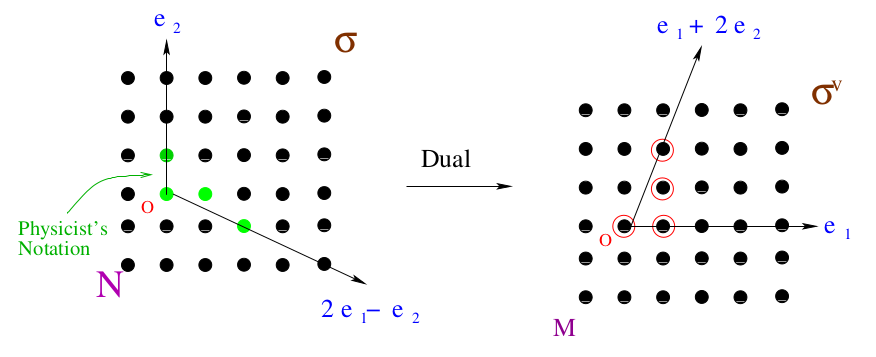
\includegraphics[scale=0.4]{Pictures/toricdiagZ2orbifold.png}
                \caption{Representations of the cone and dual cone in the lattice $\Z^2$.}
            \end{figure}

            The previous example illistrate a more genral result:
            \begin{prop*}
                All abelian orbifolds are toric varities.
            \end{prop*}
            Note that this result is not that surprising considering the general expression \eqref{eq:toricvargenform}.

            \begin{examp*}
                Let us start with $\sigma=\Cone(\{e_1,2e_1+e_2\})$. We then get $\sigma^\vee=\Cone(\{e_2,e_1-2e_2\})$ so $S_\sigma=\Span_{\Z^+}(\{e_2,e_1-2e_2\})$ and $\C[S_\sigma]=\C[y,xy^{-2}]=\C[u,v]$.
            \end{examp*}

            Now what happens with faces? An inclusion of face $\tau\subset\sigma$ gives an inclusions of the semigroups $S_\sigma\subset S_\tau$ and $\C[S_\sigma]\subset \C[S_\tau]$. This induces a morphism $U_\tau\to U_\sigma$ of affine toric varieties and it happens the this morphism is an open embedding.
            \begin{examp*}
                If $\sigma=\Cone(e_1,e_2)$ then we find $U_\sigma=\C^2$. There are three faces: $\rho_1=\Cone(e_1)$, $\rho_2=\Cone(e_2)$ and the origin $0$. These faces can be described by hyperplane $H_{e_2}, H_{e_1}$\marker and $H_{e_1+e_2}$ respectively, so we get
                \begin{align}
                    \C[S_{\rho_1}] &= \C[x,y,y^{-1}],
                    \C[S_{\rho_2}] &= \C[x,x^{-1},y],
                    \C[S_{0}] &= \C[x,y,x^{-1},y^{-1}].
                \end{align}
                They define the varieties $U_{\rho_1}=\C^*\times\C$, $U_{\rho_1}=\C\times\C^*$ and $(\C^*)^2$\marker, which are all open subvarieties of $\C^2$.
            \end{examp*}

        \subsubsection{More general construction}

            In general, an affine variety canbe defined by an ideal in $\C[x_1,\dots,x_n]$. In the same way, a toric affine variety can be defined by a \emph{toric ideal} (or \emph{binomial ideal}), i.e. an ideal in $\C[x_1,\dots,x_n]$ generated by binomials (polynoamils with precisely two non-zero coefficients).
            \begin{theorem*}
                Let $V$ be an affine variety. The following are equivalent:
                \begin{itemize}
                    \item $V$ is toric,
                    \item $V=\Spec(\C[S])$ for an affine semigroup $S$,
                    \item $V=V(I)$ for a toric ideal.
                \end{itemize}
            \end{theorem*}
            This is a very powerfull theorem since is states that an affine avariety is toric if and only if the generating polynomials of its ideal are binomials.

            %Toric varities of a cone are a way to construct toric varieties but there are others that we will not detail here.

        \subsubsection{Toric variety of a fan}
            
            A \emph{fan} is a collection $\Delta$ of cones in $N_\R$ such that each face of a cone is also a cone and the intersection of two cones is a face of each. Those two requirement imply in particular that the intersection of two cones in a fan is again a cone in the fan. Note that to any cone corresponds a fan containing the cone itself and all its faces.

            For a cone $\sigma$ in $N_\R$ the variety $U_\sigma$ contains the torus $T_N$ so fan in $N_\R$ produces a collection of varieties that all contain th same torus $T_N$. Gluing together the affine varities we obtain $X_\Delta$, it is clear that $T_N$ is an open subset of $X_\Delta$ and that $T_N$ acts on $X_\Delta$. This is called the \emph{toric variety of a fan}.

            
            For the toric varitey of a fan fan, each cone in the fan turns out to be determines an orbit $O(\sigma)$ of the torus.
            
            

            Let $\Delta$ be an $n$-dimensional fan. We denote by $\Delta(j)$ ($j\leq n$) the collection of $j$-dimensional cones in $\Delta$. 

            Let us denote by $\Delta(1)$ a set of $n$ one-dimensional cones in $N_\R$. Each cone in $\Delta(1)$ is generated by a vector of $N=\Z^m$ and we denote those generating vectors by $v_1,\dots,v_n$.

        \subsubsection{Singularities}

            A cone is said to be \emph{smooth} if it is generated by part of a lattice basis.
            \begin{theorem*}
                A cone $\sigma$ is smooth of and only if $U_\sigma$ is smooth.
            \end{theorem*}
            \begin{examp*}
                The affine toric variety $Z(x^2-y^3)$ discuss above is not smooth.
            \end{examp*}

            \begin{prop*}
                The varitey $X_\Delta$ is is non-singular if and only if $\Delta$ is a smooth fan.
            \end{prop*}


            A toric variety is nonsingular if its cones of maximal dimension are generated by a basis of the lattice. This implies that every toric variety has a resolution of singularities given by another toric variety, which can be constructed by subdividing the maximal cones into cones of non-singular toric varieties.

        

    \subsection{Calabi-Yau and non-compactness conditions}

\section{Correspondence between gauge theory and singularity}

    Above, we presented all the possible orbifold constructions of supersymmetric quiver gauge theories in four dimensions. We started from quotienting the transverse space and we found the corresponding (supersymmetric) gauge theory. In other words, we started from the singularity a found the gauge theory. We can therefore consider that the orbifold singularities are understood. However, not all singularities are orbifold one, such as the conifold for example. We can then ask ourselves how to obtain the gauge theory for more general singularities than the orbifold ones. Is a general approach possible ? On the other hand, we can also study the converse question; is it possible to to obtain the singularity from the gauge theory? And if it is, how so? In general we will see that there is a bijection between the four-dimensional supersymmetric worldvolume gauge theory and the Calabi-Yau singularity. We now detail this bijection.

    \begin{figure}[H]
        \centering
        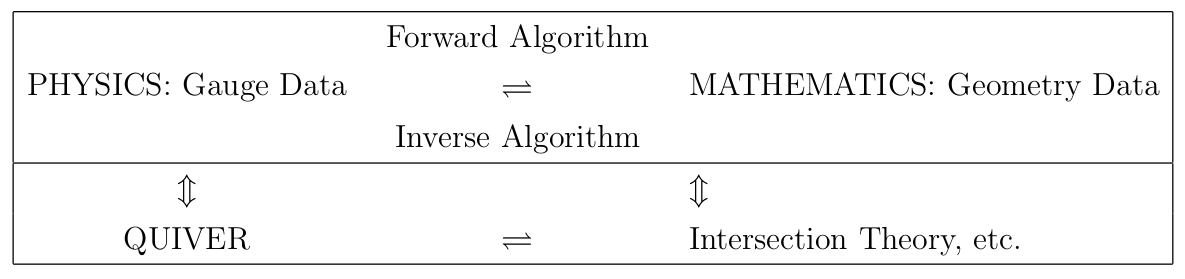
\includegraphics[scale=0.3]{Pictures/algorithm.png}
        \caption{Inverse and forward algorithm, from \cite{he2004lectures}.}
    \end{figure}

    \subsection{Gauged linear sigma model (GLSM)}

        The gauged linear sigma model provides a physical perspective on toric varieties which provides us with the right approach for the forward algorithm. Let us consider the vectorspace $\C^q$ with complex coordinates $z_1,\dots,z_q$. We provide it with a an action of $\C^{*(q-d)}$ $z_i\mapsto\lambda^{Q^a_i}z_i$ with $\lambda_a\in\C^*$ and $Q^a_i\in\Z$ ($a=1,\dots,q-d$) so $Q$ is a $q\times(q-d)$ integer matrix. So under $(\lambda_1,\dots,\lambda_{q-d})$, we have
        \begin{equation}
            \begin{bmatrix}
                z_1\\
                \vdots\\
                z_q
            \end{bmatrix}
            \mapsto
            \begin{bmatrix}
                \lambda_a
            \end{bmatrix}
            \begin{bmatrix}
                z_1\\
                \vdots\\
                z_q
            \end{bmatrix}
        \end{equation}

    \subsection{From gauge theory to singularity: forward algorithm}

        We start with the simplest question: how to recover the singularity from the gauge theory? We already mentioned that the vacuum parameter space of the scalar fields of the gauge theory is the so-called moduli space, denoted $\M$. Because our D$3$-brane is a point in the Calabi-Yau threefold, the vacuum moduli space $\M$ is the affine coordinates of the Calabi-Yau singularity $S$.

        For the ADE $\mN=2$ theories discussed in section \ref{sec:N2QGT}, by the Kronheimer-Nakajima construction \cite{Kronheimer1990}, the moduli space is a hyper-Kähler quotient. In general, the moduli space can be constructed as a \emph{quiver variety}, i.e. a variety constructed from the moduli space of quiver a quiver representation. More rpecisely, given the dimensions of the vector spaces assigned to every vertex, one can form a variety which characterizes all representations of that quiver with those specified dimensions, and consider stability conditions. Let us see some examples of this.

        The anomaly free condition is
        \begin{equation}
            (a_{ij}-a_{ji})n_i=0\marker.
        \end{equation}

    \subsection{Forward algorithm for abelina orbifolds}

        

    \subsection{From singularity to gauge theory: inverse algorithm}

        Mathematically, a quiver gauge theory is a representation of a finite quiver with relations. The labels are $\{N_i\in\Z_+\}$, they correspond to the dimension of the vector space $\{V_i\}$. The gauge group is $\prod_i\SU(N_i)$. The gauge fields are self-adjoint arrows $\Hom(V_i,V_i)$ while the matter fields are bi-fundamentals fermions/bosons and are arrows $X_{ij}\in\Hom(V_j,V_i)$. For a quiver with adjacency matrix $a_{ij}$, the gauge anomaly cancellation condition can be generally expressed as
        \begin{equation}
            (a_{ij}-a_{ji})N_i=0.
        \end{equation}
        At last, there are some relations that arises the superpotential $W(\{X_{ij}\})$. The vacuum is the minima of the superpotential. In other words,
        \begin{equation}
            \pdv{W}{X_{ij}}=0.
        \end{equation}

        \subsubsection{Application to Toric del Pezzo's}

\section{Toric duality}

\part{Beyond toric singularities}

    \begin{figure}[H]
        \centering
        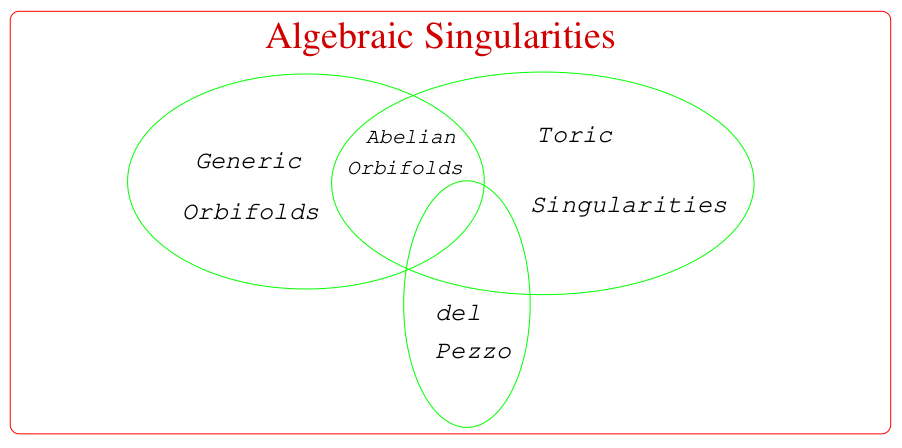
\includegraphics[scale=0.3]{Pictures/algebraicsingularities.png}
        \caption{Venn diagram of different types of algebraic singularities, from \cite{he2004lectures}.}
    \end{figure}

\section{Conifold}

\section{Non-commutative resolutions}

